\documentclass[twoside]{book}

% Packages required by doxygen
\usepackage{fixltx2e}
\usepackage{calc}
\usepackage{doxygen}
\usepackage[export]{adjustbox} % also loads graphicx
\usepackage{graphicx}
\usepackage[utf8]{inputenc}
\usepackage{makeidx}
\usepackage{multicol}
\usepackage{multirow}
\PassOptionsToPackage{warn}{textcomp}
\usepackage{textcomp}
\usepackage[nointegrals]{wasysym}
\usepackage[table]{xcolor}

% Font selection
\usepackage[T1]{fontenc}
\usepackage[scaled=.90]{helvet}
\usepackage{courier}
\usepackage{amssymb}
\usepackage{sectsty}
\renewcommand{\familydefault}{\sfdefault}
\allsectionsfont{%
  \fontseries{bc}\selectfont%
  \color{darkgray}%
}
\renewcommand{\DoxyLabelFont}{%
  \fontseries{bc}\selectfont%
  \color{darkgray}%
}
\newcommand{\+}{\discretionary{\mbox{\scriptsize$\hookleftarrow$}}{}{}}

% Page & text layout
\usepackage{geometry}
\geometry{%
  a4paper,%
  top=2.5cm,%
  bottom=2.5cm,%
  left=2.5cm,%
  right=2.5cm%
}
\tolerance=750
\hfuzz=15pt
\hbadness=750
\setlength{\emergencystretch}{15pt}
\setlength{\parindent}{0cm}
\setlength{\parskip}{3ex plus 2ex minus 2ex}
\makeatletter
\renewcommand{\paragraph}{%
  \@startsection{paragraph}{4}{0ex}{-1.0ex}{1.0ex}{%
    \normalfont\normalsize\bfseries\SS@parafont%
  }%
}
\renewcommand{\subparagraph}{%
  \@startsection{subparagraph}{5}{0ex}{-1.0ex}{1.0ex}{%
    \normalfont\normalsize\bfseries\SS@subparafont%
  }%
}
\makeatother

% Headers & footers
\usepackage{fancyhdr}
\pagestyle{fancyplain}
\fancyhead[LE]{\fancyplain{}{\bfseries\thepage}}
\fancyhead[CE]{\fancyplain{}{}}
\fancyhead[RE]{\fancyplain{}{\bfseries\leftmark}}
\fancyhead[LO]{\fancyplain{}{\bfseries\rightmark}}
\fancyhead[CO]{\fancyplain{}{}}
\fancyhead[RO]{\fancyplain{}{\bfseries\thepage}}
\fancyfoot[LE]{\fancyplain{}{}}
\fancyfoot[CE]{\fancyplain{}{}}
\fancyfoot[RE]{\fancyplain{}{\bfseries\scriptsize Generated by Doxygen }}
\fancyfoot[LO]{\fancyplain{}{\bfseries\scriptsize Generated by Doxygen }}
\fancyfoot[CO]{\fancyplain{}{}}
\fancyfoot[RO]{\fancyplain{}{}}
\renewcommand{\footrulewidth}{0.4pt}
\renewcommand{\chaptermark}[1]{%
  \markboth{#1}{}%
}
\renewcommand{\sectionmark}[1]{%
  \markright{\thesection\ #1}%
}

% Indices & bibliography
\usepackage{natbib}
\usepackage[titles]{tocloft}
\setcounter{tocdepth}{3}
\setcounter{secnumdepth}{5}
\makeindex

% Hyperlinks (required, but should be loaded last)
\usepackage{ifpdf}
\ifpdf
  \usepackage[pdftex,pagebackref=true]{hyperref}
\else
  \usepackage[ps2pdf,pagebackref=true]{hyperref}
\fi
\hypersetup{%
  colorlinks=true,%
  linkcolor=blue,%
  citecolor=blue,%
  unicode%
}

% Custom commands
\newcommand{\clearemptydoublepage}{%
  \newpage{\pagestyle{empty}\cleardoublepage}%
}

\usepackage{caption}
\captionsetup{labelsep=space,justification=centering,font={bf},singlelinecheck=off,skip=4pt,position=top}

%===== C O N T E N T S =====

\begin{document}

% Titlepage & ToC
\hypersetup{pageanchor=false,
             bookmarksnumbered=true,
             pdfencoding=unicode
            }
\pagenumbering{alph}
\begin{titlepage}
\vspace*{7cm}
\begin{center}%
{\Large Timer Driver \\[1ex]\large Version 1.\+0.\+0 }\\
\vspace*{1cm}
{\large Generated by Doxygen 1.8.13}\\
\end{center}
\end{titlepage}
\clearemptydoublepage
\pagenumbering{roman}
\tableofcontents
\clearemptydoublepage
\pagenumbering{arabic}
\hypersetup{pageanchor=true}

%--- Begin generated contents ---
\chapter{G\+P\+I\+O\+\_\+\+D\+R\+I\+V\+ER}
\label{md__home_marko__documents_embedded_workspace_gpio_driver__r_e_a_d_m_e}
\Hypertarget{md__home_marko__documents_embedded_workspace_gpio_driver__r_e_a_d_m_e}
After reading Jacob Beningo\textquotesingle{}s book, Reusable Firmware Development, I\textquotesingle{}ve decided to begin the arduous process of building my own easily portable H\+AL to use for future projects. It feels as if all I\textquotesingle{}ve been developing for ages at this point is drivers.

The general principle is as follows\+:
\begin{DoxyItemize}
\item A general \hyperlink{gpio__interface_8h}{gpio\+\_\+interface.\+h} defines the api which will be exposed to applications. It will be this file which is included by the application. It is designed in a way to be 100\% non-\/platform dependent. Changes required may be the modification of uint32\+\_\+t types to uint16\+\_\+t to match an architecture.
\item The micrcontroller specific gpio\+\_\+stm32f4xx.\+c file contains an M\+CU specific implementation of the peripheral. Accompanying it are a config .c/.h pair. These define a table of init structures for each instance of the peripheral, as well as all relevant typedefs. These files will need to be changed to port the driver. Time to port a gpio driver seems to be less than a day\textquotesingle{}s worth of work.
\item To port the driver\+: simply prepare the M\+CU specific c and config files and set \hyperlink{gpio__interface_8h}{gpio\+\_\+interface.\+h} to include the appropriate xxxxx\+\_\+config.\+h file, and exchange the source files. 
\end{DoxyItemize}
\chapter{Data Structure Index}
\section{Data Structures}
Here are the data structures with brief descriptions\+:\begin{DoxyCompactList}
\item\contentsline{section}{\hyperlink{structgpio__config__t}{gpio\+\_\+config\+\_\+t} }{\pageref{structgpio__config__t}}{}
\end{DoxyCompactList}

\chapter{File Index}
\section{File List}
Here is a list of all documented files with brief descriptions\+:\begin{DoxyCompactList}
\item\contentsline{section}{\hyperlink{gpio__interface_8h}{gpio\+\_\+interface.\+h} \\*An interface which allows for a level of modularity when using the gpio between different architectures. Usage Notes\+: To port the driver, change the include config line to point instead to the new config.\+h file you want. The config file and the interface file together should provide all definitions to implement what you need in the machine specific c implementation file }{\pageref{gpio__interface_8h}}{}
\item\contentsline{section}{\hyperlink{gpio__stm32f411_8c}{gpio\+\_\+stm32f411.\+c} \\*Machine specific implementation of gpio }{\pageref{gpio__stm32f411_8c}}{}
\item\contentsline{section}{\hyperlink{gpio__stm32f411__config_8c}{gpio\+\_\+stm32f411\+\_\+config.\+c} \\*A file defining a config table which contains all information required by gpio\+\_\+init to initialise the pins with the desired behaviour }{\pageref{gpio__stm32f411__config_8c}}{}
\item\contentsline{section}{\hyperlink{gpio__stm32f411__config_8h}{gpio\+\_\+stm32f411\+\_\+config.\+h} \\*Machine specific configuration enumerations and structures }{\pageref{gpio__stm32f411__config_8h}}{}
\end{DoxyCompactList}

\chapter{Data Structure Documentation}
\hypertarget{structgpio__config__t}{}\section{gpio\+\_\+config\+\_\+t Struct Reference}
\label{structgpio__config__t}\index{gpio\+\_\+config\+\_\+t@{gpio\+\_\+config\+\_\+t}}


{\ttfamily \#include $<$gpio\+\_\+stm32f411\+\_\+config.\+h$>$}

\subsection*{Data Fields}
\begin{DoxyCompactItemize}
\item 
\hyperlink{gpio__stm32f411__config_8h_abf6d98e99fb0fb81b56c89f29bd6120e}{gpio\+\_\+pin\+\_\+t} \hyperlink{structgpio__config__t_aa83b7f8f34af30b37ce9e23e82de5352}{pin}
\item 
\hyperlink{gpio__stm32f411__config_8h_a491a2cbfb4e94f2afcc0d5bdef2dc454}{gpio\+\_\+mode\+\_\+t} \hyperlink{structgpio__config__t_a23aeec8098631547d58a797b2ad857c1}{mode}
\item 
\hyperlink{gpio__stm32f411__config_8h_ae69599cbb4f87bfc9da21f3db8b0fe3a}{gpio\+\_\+resistor\+\_\+t} \hyperlink{structgpio__config__t_ab5a0dd08a2fc2af65242c91b9641e112}{resistor}
\item 
\hyperlink{gpio__stm32f411__config_8h_a09cae9c54cabb67e47ab4c1200b341c6}{gpio\+\_\+output\+\_\+type\+\_\+t} \hyperlink{structgpio__config__t_abebe3aee0015b70fbbbd12a796451b62}{output\+\_\+type}
\item 
\hyperlink{gpio__stm32f411__config_8h_aa8c7c905e73523d86cfed9bd45aa9495}{gpio\+\_\+output\+\_\+speed\+\_\+t} \hyperlink{structgpio__config__t_ac73298500a7a55286292448e82fcbdbf}{output\+\_\+speed}
\item 
\hyperlink{gpio__stm32f411__config_8h_ac86e130e5617ffe35f2aa1169d8a67c0}{gpio\+\_\+mux\+\_\+t} \hyperlink{structgpio__config__t_a517a0cd4125fcd45504b02d3c4a35d06}{mux}
\end{DoxyCompactItemize}


\subsection{Detailed Description}
Configuration structure holding all values needed to configure a pin. 

\subsection{Field Documentation}
\mbox{\Hypertarget{structgpio__config__t_a23aeec8098631547d58a797b2ad857c1}\label{structgpio__config__t_a23aeec8098631547d58a797b2ad857c1}} 
\index{gpio\+\_\+config\+\_\+t@{gpio\+\_\+config\+\_\+t}!mode@{mode}}
\index{mode@{mode}!gpio\+\_\+config\+\_\+t@{gpio\+\_\+config\+\_\+t}}
\subsubsection{\texorpdfstring{mode}{mode}}
{\footnotesize\ttfamily \hyperlink{gpio__stm32f411__config_8h_a491a2cbfb4e94f2afcc0d5bdef2dc454}{gpio\+\_\+mode\+\_\+t} mode}

Selected pin mode \mbox{\Hypertarget{structgpio__config__t_a517a0cd4125fcd45504b02d3c4a35d06}\label{structgpio__config__t_a517a0cd4125fcd45504b02d3c4a35d06}} 
\index{gpio\+\_\+config\+\_\+t@{gpio\+\_\+config\+\_\+t}!mux@{mux}}
\index{mux@{mux}!gpio\+\_\+config\+\_\+t@{gpio\+\_\+config\+\_\+t}}
\subsubsection{\texorpdfstring{mux}{mux}}
{\footnotesize\ttfamily \hyperlink{gpio__stm32f411__config_8h_ac86e130e5617ffe35f2aa1169d8a67c0}{gpio\+\_\+mux\+\_\+t} mux}

Multiplexer signal used to select alternate function (only relevant in AF mode) \mbox{\Hypertarget{structgpio__config__t_ac73298500a7a55286292448e82fcbdbf}\label{structgpio__config__t_ac73298500a7a55286292448e82fcbdbf}} 
\index{gpio\+\_\+config\+\_\+t@{gpio\+\_\+config\+\_\+t}!output\+\_\+speed@{output\+\_\+speed}}
\index{output\+\_\+speed@{output\+\_\+speed}!gpio\+\_\+config\+\_\+t@{gpio\+\_\+config\+\_\+t}}
\subsubsection{\texorpdfstring{output\+\_\+speed}{output\_speed}}
{\footnotesize\ttfamily \hyperlink{gpio__stm32f411__config_8h_aa8c7c905e73523d86cfed9bd45aa9495}{gpio\+\_\+output\+\_\+speed\+\_\+t} output\+\_\+speed}

Output speed (only relevant in output mode) \mbox{\Hypertarget{structgpio__config__t_abebe3aee0015b70fbbbd12a796451b62}\label{structgpio__config__t_abebe3aee0015b70fbbbd12a796451b62}} 
\index{gpio\+\_\+config\+\_\+t@{gpio\+\_\+config\+\_\+t}!output\+\_\+type@{output\+\_\+type}}
\index{output\+\_\+type@{output\+\_\+type}!gpio\+\_\+config\+\_\+t@{gpio\+\_\+config\+\_\+t}}
\subsubsection{\texorpdfstring{output\+\_\+type}{output\_type}}
{\footnotesize\ttfamily \hyperlink{gpio__stm32f411__config_8h_a09cae9c54cabb67e47ab4c1200b341c6}{gpio\+\_\+output\+\_\+type\+\_\+t} output\+\_\+type}

Output type (only relevant in output mode) \mbox{\Hypertarget{structgpio__config__t_aa83b7f8f34af30b37ce9e23e82de5352}\label{structgpio__config__t_aa83b7f8f34af30b37ce9e23e82de5352}} 
\index{gpio\+\_\+config\+\_\+t@{gpio\+\_\+config\+\_\+t}!pin@{pin}}
\index{pin@{pin}!gpio\+\_\+config\+\_\+t@{gpio\+\_\+config\+\_\+t}}
\subsubsection{\texorpdfstring{pin}{pin}}
{\footnotesize\ttfamily \hyperlink{gpio__stm32f411__config_8h_abf6d98e99fb0fb81b56c89f29bd6120e}{gpio\+\_\+pin\+\_\+t} pin}

Which pin is being configured \mbox{\Hypertarget{structgpio__config__t_ab5a0dd08a2fc2af65242c91b9641e112}\label{structgpio__config__t_ab5a0dd08a2fc2af65242c91b9641e112}} 
\index{gpio\+\_\+config\+\_\+t@{gpio\+\_\+config\+\_\+t}!resistor@{resistor}}
\index{resistor@{resistor}!gpio\+\_\+config\+\_\+t@{gpio\+\_\+config\+\_\+t}}
\subsubsection{\texorpdfstring{resistor}{resistor}}
{\footnotesize\ttfamily \hyperlink{gpio__stm32f411__config_8h_ae69599cbb4f87bfc9da21f3db8b0fe3a}{gpio\+\_\+resistor\+\_\+t} resistor}

Pull-\/ up/down selection 

The documentation for this struct was generated from the following file\+:\begin{DoxyCompactItemize}
\item 
\hyperlink{gpio__stm32f411__config_8h}{gpio\+\_\+stm32f411\+\_\+config.\+h}\end{DoxyCompactItemize}

\chapter{File Documentation}
\hypertarget{gpio__interface_8h}{}\section{gpio\+\_\+interface.\+h File Reference}
\label{gpio__interface_8h}\index{gpio\+\_\+interface.\+h@{gpio\+\_\+interface.\+h}}


An interface which allows for a level of modularity when using the gpio between different architectures. Usage Notes\+: To port the driver, change the include config line to point instead to the new config.\+h file you want. The config file and the interface file together should provide all definitions to implement what you need in the machine specific c implementation file.  


{\ttfamily \#include \char`\"{}gpio\+\_\+stm32f411\+\_\+config.\+h\char`\"{}}\newline
{\ttfamily \#include \char`\"{}assert.\+h\char`\"{}}\newline
Include dependency graph for gpio\+\_\+interface.\+h\+:\nopagebreak
\begin{figure}[H]
\begin{center}
\leavevmode
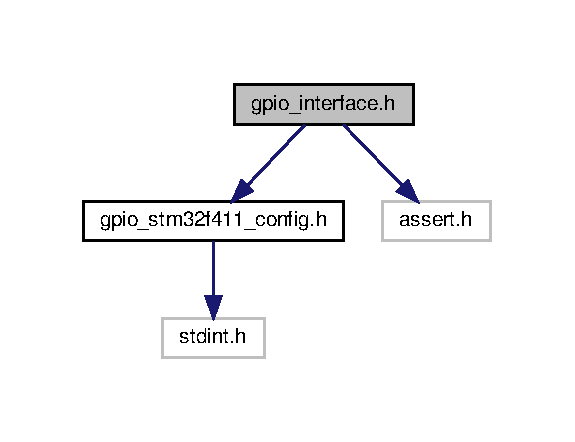
\includegraphics[width=276pt]{gpio__interface_8h__incl}
\end{center}
\end{figure}
This graph shows which files directly or indirectly include this file\+:\nopagebreak
\begin{figure}[H]
\begin{center}
\leavevmode
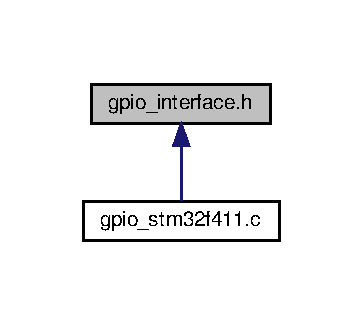
\includegraphics[width=174pt]{gpio__interface_8h__dep__incl}
\end{center}
\end{figure}
\subsection*{Functions}
\begin{DoxyCompactItemize}
\item 
void \hyperlink{gpio__interface_8h_a19bc61b9832a2879bc1c8953dcfae407}{gpio\+\_\+init} (\hyperlink{structgpio__config__t}{gpio\+\_\+config\+\_\+t} $\ast$config\+\_\+table)
\item 
\hyperlink{gpio__stm32f411__config_8h_a5e8c50a3dc51d01d0e6bdf2428ee59a7}{gpio\+\_\+pin\+\_\+state\+\_\+t} \hyperlink{gpio__interface_8h_ac793bee91b8d2c12796adcbf8ea15121}{gpio\+\_\+pin\+\_\+read} (\hyperlink{gpio__stm32f411__config_8h_abf6d98e99fb0fb81b56c89f29bd6120e}{gpio\+\_\+pin\+\_\+t} pin)
\item 
void \hyperlink{gpio__interface_8h_ac1fc916f9add814d8e48656082157d69}{gpio\+\_\+pin\+\_\+write} (\hyperlink{gpio__stm32f411__config_8h_abf6d98e99fb0fb81b56c89f29bd6120e}{gpio\+\_\+pin\+\_\+t} pin, \hyperlink{gpio__stm32f411__config_8h_a5e8c50a3dc51d01d0e6bdf2428ee59a7}{gpio\+\_\+pin\+\_\+state\+\_\+t} value)
\item 
void \hyperlink{gpio__interface_8h_aa0ddb48c46df4618795dcc007efd0865}{gpio\+\_\+pin\+\_\+toggle} (\hyperlink{gpio__stm32f411__config_8h_abf6d98e99fb0fb81b56c89f29bd6120e}{gpio\+\_\+pin\+\_\+t} pin)
\item 
void \hyperlink{gpio__interface_8h_a0578742f44243946456798e9f99b409d}{gpio\+\_\+register\+\_\+write} (uint32\+\_\+t gpio\+\_\+register, uint32\+\_\+t value)
\item 
uint32\+\_\+t \hyperlink{gpio__interface_8h_a2b37f1fe30f115d92f9d8a4aea7dc705}{gpio\+\_\+register\+\_\+read} (uint32\+\_\+t gpio\+\_\+register)
\end{DoxyCompactItemize}


\subsection{Detailed Description}
An interface which allows for a level of modularity when using the gpio between different architectures. Usage Notes\+: To port the driver, change the include config line to point instead to the new config.\+h file you want. The config file and the interface file together should provide all definitions to implement what you need in the machine specific c implementation file. 



\subsection{Function Documentation}
\mbox{\Hypertarget{gpio__interface_8h_a19bc61b9832a2879bc1c8953dcfae407}\label{gpio__interface_8h_a19bc61b9832a2879bc1c8953dcfae407}} 
\index{gpio\+\_\+interface.\+h@{gpio\+\_\+interface.\+h}!gpio\+\_\+init@{gpio\+\_\+init}}
\index{gpio\+\_\+init@{gpio\+\_\+init}!gpio\+\_\+interface.\+h@{gpio\+\_\+interface.\+h}}
\subsubsection{\texorpdfstring{gpio\+\_\+init()}{gpio\_init()}}
{\footnotesize\ttfamily void gpio\+\_\+init (\begin{DoxyParamCaption}\item[{\hyperlink{structgpio__config__t}{gpio\+\_\+config\+\_\+t} $\ast$}]{config\+\_\+table }\end{DoxyParamCaption})}

{\bfseries Description\+:} 

This function is used to initialise the gpio based on the configuration table defined in the \hyperlink{gpio__stm32f411__config_8c}{gpio\+\_\+stm32f411\+\_\+config.\+c}

P\+R\+E-\/\+C\+O\+N\+D\+I\+T\+I\+ON\+: Configuration table needs to populated (sizeof $>$ 0) ~\newline
 P\+R\+E-\/\+C\+O\+N\+D\+I\+T\+I\+ON\+: P\+I\+N\+S\+\_\+\+P\+E\+R\+\_\+\+P\+O\+RT $>$ 0 ~\newline
 P\+R\+E-\/\+C\+O\+N\+D\+I\+T\+I\+ON\+: N\+U\+M\+B\+E\+R\+\_\+\+O\+F\+\_\+\+P\+O\+R\+TS $>$ 0 ~\newline
 P\+R\+E-\/\+C\+O\+N\+D\+I\+T\+I\+ON\+: The R\+CC clocks for all planned ports must be configured and enabled.

P\+O\+S\+T-\/\+C\+O\+N\+D\+I\+T\+I\+ON\+: The G\+P\+IO is ready for use with all active pins set up.


\begin{DoxyParams}{Parameters}
{\em config\+\_\+table} & is a pointer to the configuration table that contains the initialisation structures for each planned gpio pin.\\
\hline
\end{DoxyParams}
\begin{DoxyReturn}{Returns}
void
\end{DoxyReturn}
{\bfseries Example\+:} 
\begin{DoxyCode}
\textcolor{keyword}{const} \hyperlink{structgpio__config__t}{gpio\_config\_t} *gpio\_config = \hyperlink{gpio__stm32f411__config_8c_a2f1150ba6fa738e90abcd72b16507062}{gpio\_config\_get}();
\hyperlink{gpio__interface_8h_a19bc61b9832a2879bc1c8953dcfae407}{gpio\_init}(gpio\_config);
\end{DoxyCode}


\begin{DoxySeeAlso}{See also}
\hyperlink{gpio__stm32f411__config_8h_a2f1150ba6fa738e90abcd72b16507062}{gpio\+\_\+config\+\_\+get}
\end{DoxySeeAlso}
~\newline
{\bfseries  -\/ C\+H\+A\+N\+GE H\+I\+S\+T\+O\+RY -\/ }

\tabulinesep=1mm
\begin{longtabu} spread 0pt [c]{*{4}{|X[-1]}|}
\hline
Date &Software Version &Initials &Description  \\\cline{1-4}
\end{longtabu}
~\newline
~\newline
 

 \mbox{\Hypertarget{gpio__interface_8h_ac793bee91b8d2c12796adcbf8ea15121}\label{gpio__interface_8h_ac793bee91b8d2c12796adcbf8ea15121}} 
\index{gpio\+\_\+interface.\+h@{gpio\+\_\+interface.\+h}!gpio\+\_\+pin\+\_\+read@{gpio\+\_\+pin\+\_\+read}}
\index{gpio\+\_\+pin\+\_\+read@{gpio\+\_\+pin\+\_\+read}!gpio\+\_\+interface.\+h@{gpio\+\_\+interface.\+h}}
\subsubsection{\texorpdfstring{gpio\+\_\+pin\+\_\+read()}{gpio\_pin\_read()}}
{\footnotesize\ttfamily \hyperlink{gpio__stm32f411__config_8h_a5e8c50a3dc51d01d0e6bdf2428ee59a7}{gpio\+\_\+pin\+\_\+state\+\_\+t} gpio\+\_\+pin\+\_\+read (\begin{DoxyParamCaption}\item[{\hyperlink{gpio__stm32f411__config_8h_abf6d98e99fb0fb81b56c89f29bd6120e}{gpio\+\_\+pin\+\_\+t}}]{pin }\end{DoxyParamCaption})}

{\bfseries Description\+:} 

This function reads the current state of the selected pin, regardless of whether it is in input or output mode.

P\+R\+E-\/\+C\+O\+N\+D\+I\+T\+I\+ON\+: \hyperlink{gpio__stm32f411_8c_a19bc61b9832a2879bc1c8953dcfae407}{gpio\+\_\+init()} has run successfully with the selected pin configured within the config table

P\+O\+S\+T-\/\+C\+O\+N\+D\+I\+T\+I\+ON\+: The return value contains the requested pin state in 1/0 form.


\begin{DoxyParams}{Parameters}
{\em pin} & is a member of the gpio\+\_\+pin\+\_\+t enumeration typedef\\
\hline
\end{DoxyParams}
\begin{DoxyReturn}{Returns}
gpio\+\_\+pin\+\_\+state\+\_\+t containing the pin\textquotesingle{}s current state
\end{DoxyReturn}
{\bfseries Example\+:} 


\begin{DoxyCode}
\hyperlink{gpio__stm32f411__config_8h_a5e8c50a3dc51d01d0e6bdf2428ee59a7}{gpio\_pin\_state\_t} current\_state = \hyperlink{gpio__interface_8h_ac793bee91b8d2c12796adcbf8ea15121}{gpio\_pin\_read}(GPIO\_E\_4);
\end{DoxyCode}


\begin{DoxySeeAlso}{See also}
\hyperlink{gpio__stm32f411_8c_ac1fc916f9add814d8e48656082157d69}{gpio\+\_\+pin\+\_\+write} 

\hyperlink{gpio__stm32f411_8c_aa0ddb48c46df4618795dcc007efd0865}{gpio\+\_\+pin\+\_\+toggle}
\end{DoxySeeAlso}
~\newline
{\bfseries  -\/ C\+H\+A\+N\+GE H\+I\+S\+T\+O\+RY -\/ }

\tabulinesep=1mm
\begin{longtabu} spread 0pt [c]{*{4}{|X[-1]}|}
\hline
Date &Software Version &Initials &Description  \\\cline{1-4}
\end{longtabu}
~\newline
~\newline
 

 \mbox{\Hypertarget{gpio__interface_8h_aa0ddb48c46df4618795dcc007efd0865}\label{gpio__interface_8h_aa0ddb48c46df4618795dcc007efd0865}} 
\index{gpio\+\_\+interface.\+h@{gpio\+\_\+interface.\+h}!gpio\+\_\+pin\+\_\+toggle@{gpio\+\_\+pin\+\_\+toggle}}
\index{gpio\+\_\+pin\+\_\+toggle@{gpio\+\_\+pin\+\_\+toggle}!gpio\+\_\+interface.\+h@{gpio\+\_\+interface.\+h}}
\subsubsection{\texorpdfstring{gpio\+\_\+pin\+\_\+toggle()}{gpio\_pin\_toggle()}}
{\footnotesize\ttfamily void gpio\+\_\+pin\+\_\+toggle (\begin{DoxyParamCaption}\item[{\hyperlink{gpio__stm32f411__config_8h_abf6d98e99fb0fb81b56c89f29bd6120e}{gpio\+\_\+pin\+\_\+t}}]{pin }\end{DoxyParamCaption})}

{\bfseries Description\+:} Toggles the state of the desired pin operating in output mode.

P\+R\+E-\/\+C\+O\+N\+D\+I\+T\+I\+ON\+: gpio\+\_\+init has been carried out and configured the pin in output mode.

P\+O\+S\+T-\/\+C\+O\+N\+D\+I\+T\+I\+ON\+: The pin takes on the opposite state.


\begin{DoxyParams}{Parameters}
{\em pin} & is the pin whose state we wish to change\\
\hline
\end{DoxyParams}
\begin{DoxyReturn}{Returns}
void
\end{DoxyReturn}
{\bfseries Example\+:} 


\begin{DoxyCode}
\hyperlink{gpio__interface_8h_aa0ddb48c46df4618795dcc007efd0865}{gpio\_pin\_toggle}(GPIO\_D\_15);
\end{DoxyCode}


\begin{DoxySeeAlso}{See also}
\hyperlink{gpio__stm32f411_8c_ac793bee91b8d2c12796adcbf8ea15121}{gpio\+\_\+pin\+\_\+read} 

\hyperlink{gpio__stm32f411_8c_ac1fc916f9add814d8e48656082157d69}{gpio\+\_\+pin\+\_\+write}
\end{DoxySeeAlso}
~\newline
{\bfseries  -\/ C\+H\+A\+N\+GE H\+I\+S\+T\+O\+RY -\/ }

\tabulinesep=1mm
\begin{longtabu} spread 0pt [c]{*{4}{|X[-1]}|}
\hline
Date &Software Version &Initials &Description  \\\cline{1-4}
\end{longtabu}
~\newline
~\newline
 

 \mbox{\Hypertarget{gpio__interface_8h_ac1fc916f9add814d8e48656082157d69}\label{gpio__interface_8h_ac1fc916f9add814d8e48656082157d69}} 
\index{gpio\+\_\+interface.\+h@{gpio\+\_\+interface.\+h}!gpio\+\_\+pin\+\_\+write@{gpio\+\_\+pin\+\_\+write}}
\index{gpio\+\_\+pin\+\_\+write@{gpio\+\_\+pin\+\_\+write}!gpio\+\_\+interface.\+h@{gpio\+\_\+interface.\+h}}
\subsubsection{\texorpdfstring{gpio\+\_\+pin\+\_\+write()}{gpio\_pin\_write()}}
{\footnotesize\ttfamily void gpio\+\_\+pin\+\_\+write (\begin{DoxyParamCaption}\item[{\hyperlink{gpio__stm32f411__config_8h_abf6d98e99fb0fb81b56c89f29bd6120e}{gpio\+\_\+pin\+\_\+t}}]{pin,  }\item[{\hyperlink{gpio__stm32f411__config_8h_a5e8c50a3dc51d01d0e6bdf2428ee59a7}{gpio\+\_\+pin\+\_\+state\+\_\+t}}]{value }\end{DoxyParamCaption})}

{\bfseries Description\+:} Writes the desired state to the pin operating in output mode.

P\+R\+E-\/\+C\+O\+N\+D\+I\+T\+I\+ON\+: gpio\+\_\+init has been carried out and configured the pin in output mode.

P\+O\+S\+T-\/\+C\+O\+N\+D\+I\+T\+I\+ON\+: The pin takes on the desired state.


\begin{DoxyParams}{Parameters}
{\em pin} & is the pin whose state we wish to change\\
\hline
{\em value} & is the state which we wish the pin to assume\\
\hline
\end{DoxyParams}
\begin{DoxyReturn}{Returns}
void
\end{DoxyReturn}
{\bfseries Example\+:} 


\begin{DoxyCode}
\hyperlink{gpio__interface_8h_ac1fc916f9add814d8e48656082157d69}{gpio\_pin\_write}(GPIO\_C\_0, GPIO\_PIN\_HIGH);
\end{DoxyCode}


\begin{DoxySeeAlso}{See also}
\hyperlink{gpio__stm32f411_8c_ac793bee91b8d2c12796adcbf8ea15121}{gpio\+\_\+pin\+\_\+read} 

\hyperlink{gpio__stm32f411_8c_aa0ddb48c46df4618795dcc007efd0865}{gpio\+\_\+pin\+\_\+toggle}
\end{DoxySeeAlso}
~\newline
{\bfseries  -\/ C\+H\+A\+N\+GE H\+I\+S\+T\+O\+RY -\/ }

\tabulinesep=1mm
\begin{longtabu} spread 0pt [c]{*{4}{|X[-1]}|}
\hline
Date &Software Version &Initials &Description  \\\cline{1-4}
\end{longtabu}
~\newline
~\newline
 

 \mbox{\Hypertarget{gpio__interface_8h_a2b37f1fe30f115d92f9d8a4aea7dc705}\label{gpio__interface_8h_a2b37f1fe30f115d92f9d8a4aea7dc705}} 
\index{gpio\+\_\+interface.\+h@{gpio\+\_\+interface.\+h}!gpio\+\_\+register\+\_\+read@{gpio\+\_\+register\+\_\+read}}
\index{gpio\+\_\+register\+\_\+read@{gpio\+\_\+register\+\_\+read}!gpio\+\_\+interface.\+h@{gpio\+\_\+interface.\+h}}
\subsubsection{\texorpdfstring{gpio\+\_\+register\+\_\+read()}{gpio\_register\_read()}}
{\footnotesize\ttfamily uint32\+\_\+t gpio\+\_\+register\+\_\+read (\begin{DoxyParamCaption}\item[{uint32\+\_\+t}]{gpio\+\_\+register }\end{DoxyParamCaption})}

{\bfseries Description\+:} Reads a the value of the selected G\+P\+IO register in the G\+P\+IO memory space. This function can be used within a greater super function to access more advanced features of the G\+P\+IO, such as the L\+O\+CK.

P\+R\+E-\/\+C\+O\+N\+D\+I\+T\+I\+ON\+: The value of G\+P\+I\+O\+\_\+register lies within the memory map defined region dedicated to G\+P\+IO

P\+O\+S\+T-\/\+C\+O\+N\+D\+I\+T\+I\+ON\+: The registers contents are returned


\begin{DoxyParams}{Parameters}
{\em gpio\+\_\+register} & whose contents we wish to read\\
\hline
\end{DoxyParams}
\begin{DoxyReturn}{Returns}
uint32\+\_\+t the value within the register
\end{DoxyReturn}
{\bfseries Example\+:} 


\begin{DoxyCode}
uint32\_t contents = \hyperlink{gpio__interface_8h_a2b37f1fe30f115d92f9d8a4aea7dc705}{gpio\_register\_read}(GPIOD\_BASE + 0x1CUL);
\end{DoxyCode}


\begin{DoxySeeAlso}{See also}
\hyperlink{gpio__stm32f411_8c_a0578742f44243946456798e9f99b409d}{gpio\+\_\+register\+\_\+write}
\end{DoxySeeAlso}
~\newline
{\bfseries  -\/ C\+H\+A\+N\+GE H\+I\+S\+T\+O\+RY -\/ }

\tabulinesep=1mm
\begin{longtabu} spread 0pt [c]{*{4}{|X[-1]}|}
\hline
Date &Software Version &Initials &Description  \\\cline{1-4}
\end{longtabu}
~\newline
~\newline
 

 \mbox{\Hypertarget{gpio__interface_8h_a0578742f44243946456798e9f99b409d}\label{gpio__interface_8h_a0578742f44243946456798e9f99b409d}} 
\index{gpio\+\_\+interface.\+h@{gpio\+\_\+interface.\+h}!gpio\+\_\+register\+\_\+write@{gpio\+\_\+register\+\_\+write}}
\index{gpio\+\_\+register\+\_\+write@{gpio\+\_\+register\+\_\+write}!gpio\+\_\+interface.\+h@{gpio\+\_\+interface.\+h}}
\subsubsection{\texorpdfstring{gpio\+\_\+register\+\_\+write()}{gpio\_register\_write()}}
{\footnotesize\ttfamily void gpio\+\_\+register\+\_\+write (\begin{DoxyParamCaption}\item[{uint32\+\_\+t}]{gpio\+\_\+register,  }\item[{uint32\+\_\+t}]{value }\end{DoxyParamCaption})}

{\bfseries Description\+:} Writes a desired value to the selected G\+P\+IO register in the G\+P\+IO memory space. This function can be used within a greater super function to access more advanced features of the G\+P\+IO, such as the L\+O\+CK.

P\+R\+E-\/\+C\+O\+N\+D\+I\+T\+I\+ON\+: The value of G\+P\+I\+O\+\_\+register lies within the memory map defined region dedicated to G\+P\+IO

P\+O\+S\+T-\/\+C\+O\+N\+D\+I\+T\+I\+ON\+: The register has been modified.


\begin{DoxyParams}{Parameters}
{\em gpio\+\_\+register} & is the register whose contents we wish to change\\
\hline
{\em value} & is the state which we wish the pin to assume\\
\hline
\end{DoxyParams}
\begin{DoxyReturn}{Returns}
void
\end{DoxyReturn}
{\bfseries Example\+:} 


\begin{DoxyCode}
\hyperlink{gpio__interface_8h_a0578742f44243946456798e9f99b409d}{gpio\_register\_write}(GPIOD\_BASE + 0x1CUL, 0xDEADBEEF);
\end{DoxyCode}


\begin{DoxySeeAlso}{See also}
\hyperlink{gpio__stm32f411_8c_a2b37f1fe30f115d92f9d8a4aea7dc705}{gpio\+\_\+register\+\_\+read}
\end{DoxySeeAlso}
~\newline
{\bfseries  -\/ C\+H\+A\+N\+GE H\+I\+S\+T\+O\+RY -\/ }

\tabulinesep=1mm
\begin{longtabu} spread 0pt [c]{*{4}{|X[-1]}|}
\hline
Date &Software Version &Initials &Description  \\\cline{1-4}
\end{longtabu}
~\newline
~\newline
 

 
\hypertarget{gpio__stm32f411_8c}{}\section{gpio\+\_\+stm32f411.\+c File Reference}
\label{gpio__stm32f411_8c}\index{gpio\+\_\+stm32f411.\+c@{gpio\+\_\+stm32f411.\+c}}


machine specific implementation of gpio  


{\ttfamily \#include \char`\"{}gpio\+\_\+interface.\+h\char`\"{}}\newline
{\ttfamily \#include \char`\"{}stm32f411xe.\+h\char`\"{}}\newline
Include dependency graph for gpio\+\_\+stm32f411.\+c\+:\nopagebreak
\begin{figure}[H]
\begin{center}
\leavevmode
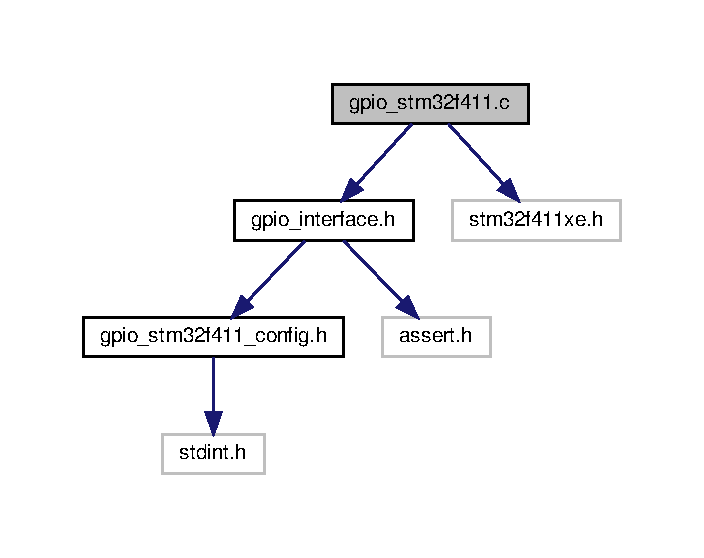
\includegraphics[width=338pt]{gpio__stm32f411_8c__incl}
\end{center}
\end{figure}
\subsection*{Macros}
\begin{DoxyCompactItemize}
\item 
\#define \hyperlink{gpio__stm32f411_8c_adb312c6a2d8064fb21620d1e141111d6}{P\+I\+N\+S\+\_\+\+P\+E\+R\+\_\+\+P\+O\+RT}~16
\item 
\#define \hyperlink{gpio__stm32f411_8c_aeb4a9e2654893b7387d045ad31b49b54}{N\+U\+M\+\_\+\+G\+P\+I\+O\+\_\+\+P\+O\+R\+TS}~N\+U\+M\+\_\+\+G\+P\+I\+O\+\_\+\+P\+I\+NS/\hyperlink{gpio__stm32f411_8c_adb312c6a2d8064fb21620d1e141111d6}{P\+I\+N\+S\+\_\+\+P\+E\+R\+\_\+\+P\+O\+RT}
\item 
\#define \hyperlink{gpio__stm32f411_8c_a5e79a132891546dc445fdb7da50aac05}{M\+O\+D\+E\+Ry\+\_\+\+W\+I\+D\+TH}~0x03\+UL
\item 
\#define \hyperlink{gpio__stm32f411_8c_a31e0afd14374afd650cad9d96f926634}{O\+T\+Y\+P\+E\+Ry\+\_\+\+W\+I\+D\+TH}~0x01\+UL
\item 
\#define \hyperlink{gpio__stm32f411_8c_a5c09cb127b6821185919edf6f073d10b}{O\+S\+P\+E\+E\+D\+Ry\+\_\+\+W\+I\+D\+TH}~0x03\+UL
\item 
\#define \hyperlink{gpio__stm32f411_8c_a5ba45c14a5628e63e7cbb11e2252ffa3}{P\+U\+P\+D\+Ry\+\_\+\+W\+I\+D\+TH}~0x03\+UL
\item 
\#define \hyperlink{gpio__stm32f411_8c_a5f7ff5c93c31db6930004969c20b6e7b}{A\+F\+L\+H\+Ry\+\_\+\+W\+I\+D\+TH}~0x0\+F\+UL
\end{DoxyCompactItemize}
\subsection*{Functions}
\begin{DoxyCompactItemize}
\item 
void \hyperlink{gpio__stm32f411_8c_a19bc61b9832a2879bc1c8953dcfae407}{gpio\+\_\+init} (\hyperlink{structgpio__config__t}{gpio\+\_\+config\+\_\+t} $\ast$config\+\_\+table)
\item 
\hyperlink{gpio__stm32f411__config_8h_a5e8c50a3dc51d01d0e6bdf2428ee59a7}{gpio\+\_\+pin\+\_\+state\+\_\+t} \hyperlink{gpio__stm32f411_8c_ac793bee91b8d2c12796adcbf8ea15121}{gpio\+\_\+pin\+\_\+read} (\hyperlink{gpio__stm32f411__config_8h_abf6d98e99fb0fb81b56c89f29bd6120e}{gpio\+\_\+pin\+\_\+t} pin)
\item 
void \hyperlink{gpio__stm32f411_8c_ac1fc916f9add814d8e48656082157d69}{gpio\+\_\+pin\+\_\+write} (\hyperlink{gpio__stm32f411__config_8h_abf6d98e99fb0fb81b56c89f29bd6120e}{gpio\+\_\+pin\+\_\+t} pin, \hyperlink{gpio__stm32f411__config_8h_a5e8c50a3dc51d01d0e6bdf2428ee59a7}{gpio\+\_\+pin\+\_\+state\+\_\+t} value)
\item 
void \hyperlink{gpio__stm32f411_8c_aa0ddb48c46df4618795dcc007efd0865}{gpio\+\_\+pin\+\_\+toggle} (\hyperlink{gpio__stm32f411__config_8h_abf6d98e99fb0fb81b56c89f29bd6120e}{gpio\+\_\+pin\+\_\+t} pin)
\item 
void \hyperlink{gpio__stm32f411_8c_a0578742f44243946456798e9f99b409d}{gpio\+\_\+register\+\_\+write} (uint32\+\_\+t gpio\+\_\+register, uint32\+\_\+t value)
\item 
uint32\+\_\+t \hyperlink{gpio__stm32f411_8c_a2b37f1fe30f115d92f9d8a4aea7dc705}{gpio\+\_\+register\+\_\+read} (uint32\+\_\+t gpio\+\_\+register)
\end{DoxyCompactItemize}
\subsection*{Variables}
\begin{DoxyCompactItemize}
\item 
const uint32\+\_\+t \hyperlink{gpio__stm32f411_8c_ac1d1f780f23cf17a4685aeeb7362e89d}{A\+C\+T\+I\+V\+E\+\_\+\+G\+P\+I\+O\+\_\+\+P\+I\+NS}
\end{DoxyCompactItemize}


\subsection{Detailed Description}
machine specific implementation of gpio 



\subsection{Macro Definition Documentation}
\mbox{\Hypertarget{gpio__stm32f411_8c_a5f7ff5c93c31db6930004969c20b6e7b}\label{gpio__stm32f411_8c_a5f7ff5c93c31db6930004969c20b6e7b}} 
\index{gpio\+\_\+stm32f411.\+c@{gpio\+\_\+stm32f411.\+c}!A\+F\+L\+H\+Ry\+\_\+\+W\+I\+D\+TH@{A\+F\+L\+H\+Ry\+\_\+\+W\+I\+D\+TH}}
\index{A\+F\+L\+H\+Ry\+\_\+\+W\+I\+D\+TH@{A\+F\+L\+H\+Ry\+\_\+\+W\+I\+D\+TH}!gpio\+\_\+stm32f411.\+c@{gpio\+\_\+stm32f411.\+c}}
\subsubsection{\texorpdfstring{A\+F\+L\+H\+Ry\+\_\+\+W\+I\+D\+TH}{AFLHRy\_WIDTH}}
{\footnotesize\ttfamily \#define A\+F\+L\+H\+Ry\+\_\+\+W\+I\+D\+TH~0x0\+F\+UL}

The width of a the bitfield controlling the alternate function M\+UX \mbox{\Hypertarget{gpio__stm32f411_8c_a5e79a132891546dc445fdb7da50aac05}\label{gpio__stm32f411_8c_a5e79a132891546dc445fdb7da50aac05}} 
\index{gpio\+\_\+stm32f411.\+c@{gpio\+\_\+stm32f411.\+c}!M\+O\+D\+E\+Ry\+\_\+\+W\+I\+D\+TH@{M\+O\+D\+E\+Ry\+\_\+\+W\+I\+D\+TH}}
\index{M\+O\+D\+E\+Ry\+\_\+\+W\+I\+D\+TH@{M\+O\+D\+E\+Ry\+\_\+\+W\+I\+D\+TH}!gpio\+\_\+stm32f411.\+c@{gpio\+\_\+stm32f411.\+c}}
\subsubsection{\texorpdfstring{M\+O\+D\+E\+Ry\+\_\+\+W\+I\+D\+TH}{MODERy\_WIDTH}}
{\footnotesize\ttfamily \#define M\+O\+D\+E\+Ry\+\_\+\+W\+I\+D\+TH~0x03\+UL}

The width of the bitfield controlling a pin\textquotesingle{}s mode \mbox{\Hypertarget{gpio__stm32f411_8c_aeb4a9e2654893b7387d045ad31b49b54}\label{gpio__stm32f411_8c_aeb4a9e2654893b7387d045ad31b49b54}} 
\index{gpio\+\_\+stm32f411.\+c@{gpio\+\_\+stm32f411.\+c}!N\+U\+M\+\_\+\+G\+P\+I\+O\+\_\+\+P\+O\+R\+TS@{N\+U\+M\+\_\+\+G\+P\+I\+O\+\_\+\+P\+O\+R\+TS}}
\index{N\+U\+M\+\_\+\+G\+P\+I\+O\+\_\+\+P\+O\+R\+TS@{N\+U\+M\+\_\+\+G\+P\+I\+O\+\_\+\+P\+O\+R\+TS}!gpio\+\_\+stm32f411.\+c@{gpio\+\_\+stm32f411.\+c}}
\subsubsection{\texorpdfstring{N\+U\+M\+\_\+\+G\+P\+I\+O\+\_\+\+P\+O\+R\+TS}{NUM\_GPIO\_PORTS}}
{\footnotesize\ttfamily \#define N\+U\+M\+\_\+\+G\+P\+I\+O\+\_\+\+P\+O\+R\+TS~N\+U\+M\+\_\+\+G\+P\+I\+O\+\_\+\+P\+I\+NS/\hyperlink{gpio__stm32f411_8c_adb312c6a2d8064fb21620d1e141111d6}{P\+I\+N\+S\+\_\+\+P\+E\+R\+\_\+\+P\+O\+RT}}

Number of letter named ports \mbox{\Hypertarget{gpio__stm32f411_8c_a5c09cb127b6821185919edf6f073d10b}\label{gpio__stm32f411_8c_a5c09cb127b6821185919edf6f073d10b}} 
\index{gpio\+\_\+stm32f411.\+c@{gpio\+\_\+stm32f411.\+c}!O\+S\+P\+E\+E\+D\+Ry\+\_\+\+W\+I\+D\+TH@{O\+S\+P\+E\+E\+D\+Ry\+\_\+\+W\+I\+D\+TH}}
\index{O\+S\+P\+E\+E\+D\+Ry\+\_\+\+W\+I\+D\+TH@{O\+S\+P\+E\+E\+D\+Ry\+\_\+\+W\+I\+D\+TH}!gpio\+\_\+stm32f411.\+c@{gpio\+\_\+stm32f411.\+c}}
\subsubsection{\texorpdfstring{O\+S\+P\+E\+E\+D\+Ry\+\_\+\+W\+I\+D\+TH}{OSPEEDRy\_WIDTH}}
{\footnotesize\ttfamily \#define O\+S\+P\+E\+E\+D\+Ry\+\_\+\+W\+I\+D\+TH~0x03\+UL}

The width of the bitfield controlling the output speed of a pin \mbox{\Hypertarget{gpio__stm32f411_8c_a31e0afd14374afd650cad9d96f926634}\label{gpio__stm32f411_8c_a31e0afd14374afd650cad9d96f926634}} 
\index{gpio\+\_\+stm32f411.\+c@{gpio\+\_\+stm32f411.\+c}!O\+T\+Y\+P\+E\+Ry\+\_\+\+W\+I\+D\+TH@{O\+T\+Y\+P\+E\+Ry\+\_\+\+W\+I\+D\+TH}}
\index{O\+T\+Y\+P\+E\+Ry\+\_\+\+W\+I\+D\+TH@{O\+T\+Y\+P\+E\+Ry\+\_\+\+W\+I\+D\+TH}!gpio\+\_\+stm32f411.\+c@{gpio\+\_\+stm32f411.\+c}}
\subsubsection{\texorpdfstring{O\+T\+Y\+P\+E\+Ry\+\_\+\+W\+I\+D\+TH}{OTYPERy\_WIDTH}}
{\footnotesize\ttfamily \#define O\+T\+Y\+P\+E\+Ry\+\_\+\+W\+I\+D\+TH~0x01\+UL}

The width of the bitfield controlling the output type of a pin \mbox{\Hypertarget{gpio__stm32f411_8c_adb312c6a2d8064fb21620d1e141111d6}\label{gpio__stm32f411_8c_adb312c6a2d8064fb21620d1e141111d6}} 
\index{gpio\+\_\+stm32f411.\+c@{gpio\+\_\+stm32f411.\+c}!P\+I\+N\+S\+\_\+\+P\+E\+R\+\_\+\+P\+O\+RT@{P\+I\+N\+S\+\_\+\+P\+E\+R\+\_\+\+P\+O\+RT}}
\index{P\+I\+N\+S\+\_\+\+P\+E\+R\+\_\+\+P\+O\+RT@{P\+I\+N\+S\+\_\+\+P\+E\+R\+\_\+\+P\+O\+RT}!gpio\+\_\+stm32f411.\+c@{gpio\+\_\+stm32f411.\+c}}
\subsubsection{\texorpdfstring{P\+I\+N\+S\+\_\+\+P\+E\+R\+\_\+\+P\+O\+RT}{PINS\_PER\_PORT}}
{\footnotesize\ttfamily \#define P\+I\+N\+S\+\_\+\+P\+E\+R\+\_\+\+P\+O\+RT~16}

The number of pins per letter named port \mbox{\Hypertarget{gpio__stm32f411_8c_a5ba45c14a5628e63e7cbb11e2252ffa3}\label{gpio__stm32f411_8c_a5ba45c14a5628e63e7cbb11e2252ffa3}} 
\index{gpio\+\_\+stm32f411.\+c@{gpio\+\_\+stm32f411.\+c}!P\+U\+P\+D\+Ry\+\_\+\+W\+I\+D\+TH@{P\+U\+P\+D\+Ry\+\_\+\+W\+I\+D\+TH}}
\index{P\+U\+P\+D\+Ry\+\_\+\+W\+I\+D\+TH@{P\+U\+P\+D\+Ry\+\_\+\+W\+I\+D\+TH}!gpio\+\_\+stm32f411.\+c@{gpio\+\_\+stm32f411.\+c}}
\subsubsection{\texorpdfstring{P\+U\+P\+D\+Ry\+\_\+\+W\+I\+D\+TH}{PUPDRy\_WIDTH}}
{\footnotesize\ttfamily \#define P\+U\+P\+D\+Ry\+\_\+\+W\+I\+D\+TH~0x03\+UL}

The width of the bitfield controlling pull up/pull down selection 

\subsection{Function Documentation}
\mbox{\Hypertarget{gpio__stm32f411_8c_a19bc61b9832a2879bc1c8953dcfae407}\label{gpio__stm32f411_8c_a19bc61b9832a2879bc1c8953dcfae407}} 
\index{gpio\+\_\+stm32f411.\+c@{gpio\+\_\+stm32f411.\+c}!gpio\+\_\+init@{gpio\+\_\+init}}
\index{gpio\+\_\+init@{gpio\+\_\+init}!gpio\+\_\+stm32f411.\+c@{gpio\+\_\+stm32f411.\+c}}
\subsubsection{\texorpdfstring{gpio\+\_\+init()}{gpio\_init()}}
{\footnotesize\ttfamily void gpio\+\_\+init (\begin{DoxyParamCaption}\item[{\hyperlink{structgpio__config__t}{gpio\+\_\+config\+\_\+t} $\ast$}]{config\+\_\+table }\end{DoxyParamCaption})}

{\bfseries Description\+:} 

This function is used to initialise the gpio based on the configuration table defined in the \hyperlink{gpio__stm32f411__config_8c}{gpio\+\_\+stm32f411\+\_\+config.\+c}

P\+R\+E-\/\+C\+O\+N\+D\+I\+T\+I\+ON\+: Configuration table needs to populated (sizeof $>$ 0) ~\newline
 P\+R\+E-\/\+C\+O\+N\+D\+I\+T\+I\+ON\+: P\+I\+N\+S\+\_\+\+P\+E\+R\+\_\+\+P\+O\+RT $>$ 0 ~\newline
 P\+R\+E-\/\+C\+O\+N\+D\+I\+T\+I\+ON\+: N\+U\+M\+B\+E\+R\+\_\+\+O\+F\+\_\+\+P\+O\+R\+TS $>$ 0 ~\newline
 P\+R\+E-\/\+C\+O\+N\+D\+I\+T\+I\+ON\+: The R\+CC clocks for all planned ports must be configured and enabled.

P\+O\+S\+T-\/\+C\+O\+N\+D\+I\+T\+I\+ON\+: The G\+P\+IO is ready for use with all active pins set up.


\begin{DoxyParams}{Parameters}
{\em config\+\_\+table} & is a pointer to the configuration table that contains the initialisation structures for each planned gpio pin.\\
\hline
\end{DoxyParams}
\begin{DoxyReturn}{Returns}
void
\end{DoxyReturn}
{\bfseries Example\+:} 
\begin{DoxyCode}
\textcolor{keyword}{const} \hyperlink{structgpio__config__t}{gpio\_config\_t} *gpio\_config = \hyperlink{gpio__stm32f411__config_8c_a2f1150ba6fa738e90abcd72b16507062}{gpio\_config\_get}();
\hyperlink{gpio__interface_8h_a19bc61b9832a2879bc1c8953dcfae407}{gpio\_init}(gpio\_config);
\end{DoxyCode}


\begin{DoxySeeAlso}{See also}
\hyperlink{gpio__stm32f411__config_8h_a2f1150ba6fa738e90abcd72b16507062}{gpio\+\_\+config\+\_\+get}
\end{DoxySeeAlso}
~\newline
{\bfseries  -\/ C\+H\+A\+N\+GE H\+I\+S\+T\+O\+RY -\/ }

\tabulinesep=1mm
\begin{longtabu} spread 0pt [c]{*{4}{|X[-1]}|}
\hline
Date &Software Version &Initials &Description  \\\cline{1-4}
\end{longtabu}
~\newline
~\newline
 

 \mbox{\Hypertarget{gpio__stm32f411_8c_ac793bee91b8d2c12796adcbf8ea15121}\label{gpio__stm32f411_8c_ac793bee91b8d2c12796adcbf8ea15121}} 
\index{gpio\+\_\+stm32f411.\+c@{gpio\+\_\+stm32f411.\+c}!gpio\+\_\+pin\+\_\+read@{gpio\+\_\+pin\+\_\+read}}
\index{gpio\+\_\+pin\+\_\+read@{gpio\+\_\+pin\+\_\+read}!gpio\+\_\+stm32f411.\+c@{gpio\+\_\+stm32f411.\+c}}
\subsubsection{\texorpdfstring{gpio\+\_\+pin\+\_\+read()}{gpio\_pin\_read()}}
{\footnotesize\ttfamily \hyperlink{gpio__stm32f411__config_8h_a5e8c50a3dc51d01d0e6bdf2428ee59a7}{gpio\+\_\+pin\+\_\+state\+\_\+t} gpio\+\_\+pin\+\_\+read (\begin{DoxyParamCaption}\item[{\hyperlink{gpio__stm32f411__config_8h_abf6d98e99fb0fb81b56c89f29bd6120e}{gpio\+\_\+pin\+\_\+t}}]{pin }\end{DoxyParamCaption})}

{\bfseries Description\+:} 

This function reads the current state of the selected pin, regardless of whether it is in input or output mode.

P\+R\+E-\/\+C\+O\+N\+D\+I\+T\+I\+ON\+: \hyperlink{gpio__stm32f411_8c_a19bc61b9832a2879bc1c8953dcfae407}{gpio\+\_\+init()} has run successfully with the selected pin configured within the config table

P\+O\+S\+T-\/\+C\+O\+N\+D\+I\+T\+I\+ON\+: The return value contains the requested pin state in 1/0 form.


\begin{DoxyParams}{Parameters}
{\em pin} & is a member of the gpio\+\_\+pin\+\_\+t enumeration typedef\\
\hline
\end{DoxyParams}
\begin{DoxyReturn}{Returns}
gpio\+\_\+pin\+\_\+state\+\_\+t containing the pin\textquotesingle{}s current state
\end{DoxyReturn}
{\bfseries Example\+:} 


\begin{DoxyCode}
\hyperlink{gpio__stm32f411__config_8h_a5e8c50a3dc51d01d0e6bdf2428ee59a7}{gpio\_pin\_state\_t} current\_state = \hyperlink{gpio__interface_8h_ac793bee91b8d2c12796adcbf8ea15121}{gpio\_pin\_read}(GPIO\_E\_4);
\end{DoxyCode}


\begin{DoxySeeAlso}{See also}
\hyperlink{gpio__stm32f411_8c_ac1fc916f9add814d8e48656082157d69}{gpio\+\_\+pin\+\_\+write} 

\hyperlink{gpio__stm32f411_8c_aa0ddb48c46df4618795dcc007efd0865}{gpio\+\_\+pin\+\_\+toggle}
\end{DoxySeeAlso}
~\newline
{\bfseries  -\/ C\+H\+A\+N\+GE H\+I\+S\+T\+O\+RY -\/ }

\tabulinesep=1mm
\begin{longtabu} spread 0pt [c]{*{4}{|X[-1]}|}
\hline
Date &Software Version &Initials &Description  \\\cline{1-4}
\end{longtabu}
~\newline
~\newline
 

 \mbox{\Hypertarget{gpio__stm32f411_8c_aa0ddb48c46df4618795dcc007efd0865}\label{gpio__stm32f411_8c_aa0ddb48c46df4618795dcc007efd0865}} 
\index{gpio\+\_\+stm32f411.\+c@{gpio\+\_\+stm32f411.\+c}!gpio\+\_\+pin\+\_\+toggle@{gpio\+\_\+pin\+\_\+toggle}}
\index{gpio\+\_\+pin\+\_\+toggle@{gpio\+\_\+pin\+\_\+toggle}!gpio\+\_\+stm32f411.\+c@{gpio\+\_\+stm32f411.\+c}}
\subsubsection{\texorpdfstring{gpio\+\_\+pin\+\_\+toggle()}{gpio\_pin\_toggle()}}
{\footnotesize\ttfamily void gpio\+\_\+pin\+\_\+toggle (\begin{DoxyParamCaption}\item[{\hyperlink{gpio__stm32f411__config_8h_abf6d98e99fb0fb81b56c89f29bd6120e}{gpio\+\_\+pin\+\_\+t}}]{pin }\end{DoxyParamCaption})}

{\bfseries Description\+:} Toggles the state of the desired pin operating in output mode.

P\+R\+E-\/\+C\+O\+N\+D\+I\+T\+I\+ON\+: gpio\+\_\+init has been carried out and configured the pin in output mode.

P\+O\+S\+T-\/\+C\+O\+N\+D\+I\+T\+I\+ON\+: The pin takes on the opposite state.


\begin{DoxyParams}{Parameters}
{\em pin} & is the pin whose state we wish to change\\
\hline
\end{DoxyParams}
\begin{DoxyReturn}{Returns}
void
\end{DoxyReturn}
{\bfseries Example\+:} 


\begin{DoxyCode}
\hyperlink{gpio__interface_8h_aa0ddb48c46df4618795dcc007efd0865}{gpio\_pin\_toggle}(GPIO\_D\_15);
\end{DoxyCode}


\begin{DoxySeeAlso}{See also}
\hyperlink{gpio__stm32f411_8c_ac793bee91b8d2c12796adcbf8ea15121}{gpio\+\_\+pin\+\_\+read} 

\hyperlink{gpio__stm32f411_8c_ac1fc916f9add814d8e48656082157d69}{gpio\+\_\+pin\+\_\+write}
\end{DoxySeeAlso}
~\newline
{\bfseries  -\/ C\+H\+A\+N\+GE H\+I\+S\+T\+O\+RY -\/ }

\tabulinesep=1mm
\begin{longtabu} spread 0pt [c]{*{4}{|X[-1]}|}
\hline
Date &Software Version &Initials &Description  \\\cline{1-4}
\end{longtabu}
~\newline
~\newline
 

 \mbox{\Hypertarget{gpio__stm32f411_8c_ac1fc916f9add814d8e48656082157d69}\label{gpio__stm32f411_8c_ac1fc916f9add814d8e48656082157d69}} 
\index{gpio\+\_\+stm32f411.\+c@{gpio\+\_\+stm32f411.\+c}!gpio\+\_\+pin\+\_\+write@{gpio\+\_\+pin\+\_\+write}}
\index{gpio\+\_\+pin\+\_\+write@{gpio\+\_\+pin\+\_\+write}!gpio\+\_\+stm32f411.\+c@{gpio\+\_\+stm32f411.\+c}}
\subsubsection{\texorpdfstring{gpio\+\_\+pin\+\_\+write()}{gpio\_pin\_write()}}
{\footnotesize\ttfamily void gpio\+\_\+pin\+\_\+write (\begin{DoxyParamCaption}\item[{\hyperlink{gpio__stm32f411__config_8h_abf6d98e99fb0fb81b56c89f29bd6120e}{gpio\+\_\+pin\+\_\+t}}]{pin,  }\item[{\hyperlink{gpio__stm32f411__config_8h_a5e8c50a3dc51d01d0e6bdf2428ee59a7}{gpio\+\_\+pin\+\_\+state\+\_\+t}}]{value }\end{DoxyParamCaption})}

{\bfseries Description\+:} Writes the desired state to the pin operating in output mode.

P\+R\+E-\/\+C\+O\+N\+D\+I\+T\+I\+ON\+: gpio\+\_\+init has been carried out and configured the pin in output mode.

P\+O\+S\+T-\/\+C\+O\+N\+D\+I\+T\+I\+ON\+: The pin takes on the desired state.


\begin{DoxyParams}{Parameters}
{\em pin} & is the pin whose state we wish to change\\
\hline
{\em value} & is the state which we wish the pin to assume\\
\hline
\end{DoxyParams}
\begin{DoxyReturn}{Returns}
void
\end{DoxyReturn}
{\bfseries Example\+:} 


\begin{DoxyCode}
\hyperlink{gpio__interface_8h_ac1fc916f9add814d8e48656082157d69}{gpio\_pin\_write}(GPIO\_C\_0, GPIO\_PIN\_HIGH);
\end{DoxyCode}


\begin{DoxySeeAlso}{See also}
\hyperlink{gpio__stm32f411_8c_ac793bee91b8d2c12796adcbf8ea15121}{gpio\+\_\+pin\+\_\+read} 

\hyperlink{gpio__stm32f411_8c_aa0ddb48c46df4618795dcc007efd0865}{gpio\+\_\+pin\+\_\+toggle}
\end{DoxySeeAlso}
~\newline
{\bfseries  -\/ C\+H\+A\+N\+GE H\+I\+S\+T\+O\+RY -\/ }

\tabulinesep=1mm
\begin{longtabu} spread 0pt [c]{*{4}{|X[-1]}|}
\hline
Date &Software Version &Initials &Description  \\\cline{1-4}
\end{longtabu}
~\newline
~\newline
 

 \mbox{\Hypertarget{gpio__stm32f411_8c_a2b37f1fe30f115d92f9d8a4aea7dc705}\label{gpio__stm32f411_8c_a2b37f1fe30f115d92f9d8a4aea7dc705}} 
\index{gpio\+\_\+stm32f411.\+c@{gpio\+\_\+stm32f411.\+c}!gpio\+\_\+register\+\_\+read@{gpio\+\_\+register\+\_\+read}}
\index{gpio\+\_\+register\+\_\+read@{gpio\+\_\+register\+\_\+read}!gpio\+\_\+stm32f411.\+c@{gpio\+\_\+stm32f411.\+c}}
\subsubsection{\texorpdfstring{gpio\+\_\+register\+\_\+read()}{gpio\_register\_read()}}
{\footnotesize\ttfamily uint32\+\_\+t gpio\+\_\+register\+\_\+read (\begin{DoxyParamCaption}\item[{uint32\+\_\+t}]{gpio\+\_\+register }\end{DoxyParamCaption})}

{\bfseries Description\+:} Reads a the value of the selected G\+P\+IO register in the G\+P\+IO memory space. This function can be used within a greater super function to access more advanced features of the G\+P\+IO, such as the L\+O\+CK.

P\+R\+E-\/\+C\+O\+N\+D\+I\+T\+I\+ON\+: The value of G\+P\+I\+O\+\_\+register lies within the memory map defined region dedicated to G\+P\+IO

P\+O\+S\+T-\/\+C\+O\+N\+D\+I\+T\+I\+ON\+: The registers contents are returned


\begin{DoxyParams}{Parameters}
{\em gpio\+\_\+register} & whose contents we wish to read\\
\hline
\end{DoxyParams}
\begin{DoxyReturn}{Returns}
uint32\+\_\+t the value within the register
\end{DoxyReturn}
{\bfseries Example\+:} 


\begin{DoxyCode}
uint32\_t contents = \hyperlink{gpio__interface_8h_a2b37f1fe30f115d92f9d8a4aea7dc705}{gpio\_register\_read}(GPIOD\_BASE + 0x1CUL);
\end{DoxyCode}


\begin{DoxySeeAlso}{See also}
\hyperlink{gpio__stm32f411_8c_a0578742f44243946456798e9f99b409d}{gpio\+\_\+register\+\_\+write}
\end{DoxySeeAlso}
~\newline
{\bfseries  -\/ C\+H\+A\+N\+GE H\+I\+S\+T\+O\+RY -\/ }

\tabulinesep=1mm
\begin{longtabu} spread 0pt [c]{*{4}{|X[-1]}|}
\hline
Date &Software Version &Initials &Description  \\\cline{1-4}
\end{longtabu}
~\newline
~\newline
 

 \mbox{\Hypertarget{gpio__stm32f411_8c_a0578742f44243946456798e9f99b409d}\label{gpio__stm32f411_8c_a0578742f44243946456798e9f99b409d}} 
\index{gpio\+\_\+stm32f411.\+c@{gpio\+\_\+stm32f411.\+c}!gpio\+\_\+register\+\_\+write@{gpio\+\_\+register\+\_\+write}}
\index{gpio\+\_\+register\+\_\+write@{gpio\+\_\+register\+\_\+write}!gpio\+\_\+stm32f411.\+c@{gpio\+\_\+stm32f411.\+c}}
\subsubsection{\texorpdfstring{gpio\+\_\+register\+\_\+write()}{gpio\_register\_write()}}
{\footnotesize\ttfamily void gpio\+\_\+register\+\_\+write (\begin{DoxyParamCaption}\item[{uint32\+\_\+t}]{gpio\+\_\+register,  }\item[{uint32\+\_\+t}]{value }\end{DoxyParamCaption})}

{\bfseries Description\+:} Writes a desired value to the selected G\+P\+IO register in the G\+P\+IO memory space. This function can be used within a greater super function to access more advanced features of the G\+P\+IO, such as the L\+O\+CK.

P\+R\+E-\/\+C\+O\+N\+D\+I\+T\+I\+ON\+: The value of G\+P\+I\+O\+\_\+register lies within the memory map defined region dedicated to G\+P\+IO

P\+O\+S\+T-\/\+C\+O\+N\+D\+I\+T\+I\+ON\+: The register has been modified.


\begin{DoxyParams}{Parameters}
{\em gpio\+\_\+register} & is the register whose contents we wish to change\\
\hline
{\em value} & is the state which we wish the pin to assume\\
\hline
\end{DoxyParams}
\begin{DoxyReturn}{Returns}
void
\end{DoxyReturn}
{\bfseries Example\+:} 


\begin{DoxyCode}
\hyperlink{gpio__interface_8h_a0578742f44243946456798e9f99b409d}{gpio\_register\_write}(GPIOD\_BASE + 0x1CUL, 0xDEADBEEF);
\end{DoxyCode}


\begin{DoxySeeAlso}{See also}
\hyperlink{gpio__stm32f411_8c_a2b37f1fe30f115d92f9d8a4aea7dc705}{gpio\+\_\+register\+\_\+read}
\end{DoxySeeAlso}
~\newline
{\bfseries  -\/ C\+H\+A\+N\+GE H\+I\+S\+T\+O\+RY -\/ }

\tabulinesep=1mm
\begin{longtabu} spread 0pt [c]{*{4}{|X[-1]}|}
\hline
Date &Software Version &Initials &Description  \\\cline{1-4}
\end{longtabu}
~\newline
~\newline
 

 

\subsection{Variable Documentation}
\mbox{\Hypertarget{gpio__stm32f411_8c_ac1d1f780f23cf17a4685aeeb7362e89d}\label{gpio__stm32f411_8c_ac1d1f780f23cf17a4685aeeb7362e89d}} 
\index{gpio\+\_\+stm32f411.\+c@{gpio\+\_\+stm32f411.\+c}!A\+C\+T\+I\+V\+E\+\_\+\+G\+P\+I\+O\+\_\+\+P\+I\+NS@{A\+C\+T\+I\+V\+E\+\_\+\+G\+P\+I\+O\+\_\+\+P\+I\+NS}}
\index{A\+C\+T\+I\+V\+E\+\_\+\+G\+P\+I\+O\+\_\+\+P\+I\+NS@{A\+C\+T\+I\+V\+E\+\_\+\+G\+P\+I\+O\+\_\+\+P\+I\+NS}!gpio\+\_\+stm32f411.\+c@{gpio\+\_\+stm32f411.\+c}}
\subsubsection{\texorpdfstring{A\+C\+T\+I\+V\+E\+\_\+\+G\+P\+I\+O\+\_\+\+P\+I\+NS}{ACTIVE\_GPIO\_PINS}}
{\footnotesize\ttfamily const uint32\+\_\+t A\+C\+T\+I\+V\+E\+\_\+\+G\+P\+I\+O\+\_\+\+P\+I\+NS}

Prevents iteration over 64 pins when only a few are used 
\hypertarget{gpio__stm32f411__config_8c}{}\section{gpio\+\_\+stm32f411\+\_\+config.\+c File Reference}
\label{gpio__stm32f411__config_8c}\index{gpio\+\_\+stm32f411\+\_\+config.\+c@{gpio\+\_\+stm32f411\+\_\+config.\+c}}


A file defining a config table which contains all information required by gpio\+\_\+init to initialise the pins with the desired behaviour.  


{\ttfamily \#include \char`\"{}gpio\+\_\+stm32f411\+\_\+config.\+h\char`\"{}}\newline
Include dependency graph for gpio\+\_\+stm32f411\+\_\+config.\+c\+:\nopagebreak
\begin{figure}[H]
\begin{center}
\leavevmode
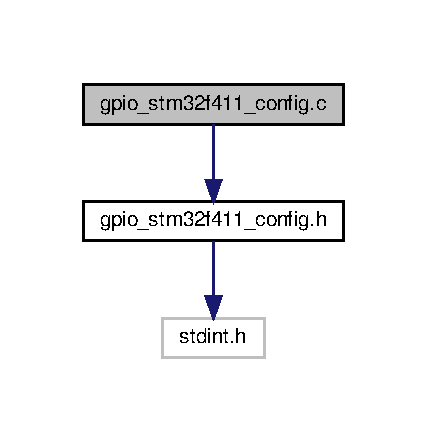
\includegraphics[width=205pt]{gpio__stm32f411__config_8c__incl}
\end{center}
\end{figure}
\subsection*{Functions}
\begin{DoxyCompactItemize}
\item 
const \hyperlink{structgpio__config__t}{gpio\+\_\+config\+\_\+t} $\ast$ \hyperlink{gpio__stm32f411__config_8c_a2f1150ba6fa738e90abcd72b16507062}{gpio\+\_\+config\+\_\+get} (void)
\end{DoxyCompactItemize}
\subsection*{Variables}
\begin{DoxyCompactItemize}
\item 
const uint32\+\_\+t \hyperlink{gpio__stm32f411__config_8c_ac1d1f780f23cf17a4685aeeb7362e89d}{A\+C\+T\+I\+V\+E\+\_\+\+G\+P\+I\+O\+\_\+\+P\+I\+NS} = sizeof(gpio\+\_\+config\+\_\+table)/sizeof(\hyperlink{structgpio__config__t}{gpio\+\_\+config\+\_\+t})
\end{DoxyCompactItemize}


\subsection{Detailed Description}
A file defining a config table which contains all information required by gpio\+\_\+init to initialise the pins with the desired behaviour. 



\subsection{Function Documentation}
\mbox{\Hypertarget{gpio__stm32f411__config_8c_a2f1150ba6fa738e90abcd72b16507062}\label{gpio__stm32f411__config_8c_a2f1150ba6fa738e90abcd72b16507062}} 
\index{gpio\+\_\+stm32f411\+\_\+config.\+c@{gpio\+\_\+stm32f411\+\_\+config.\+c}!gpio\+\_\+config\+\_\+get@{gpio\+\_\+config\+\_\+get}}
\index{gpio\+\_\+config\+\_\+get@{gpio\+\_\+config\+\_\+get}!gpio\+\_\+stm32f411\+\_\+config.\+c@{gpio\+\_\+stm32f411\+\_\+config.\+c}}
\subsubsection{\texorpdfstring{gpio\+\_\+config\+\_\+get()}{gpio\_config\_get()}}
{\footnotesize\ttfamily const \hyperlink{structgpio__config__t}{gpio\+\_\+config\+\_\+t}$\ast$ gpio\+\_\+config\+\_\+get (\begin{DoxyParamCaption}\item[{void}]{ }\end{DoxyParamCaption})}

{\bfseries Description\+:} Retrieves the config table for the gpio peripheral, normally hidden statically within the config.\+c file.

P\+R\+E-\/\+C\+O\+N\+D\+I\+T\+I\+ON\+: The config table has been populated/exists with a size greater than 0.

P\+O\+S\+T-\/\+C\+O\+N\+D\+I\+T\+I\+ON\+: The returned value points to the base of the config table

\begin{DoxyReturn}{Returns}
const \hyperlink{structgpio__config__t}{gpio\+\_\+config\+\_\+t} $\ast$
\end{DoxyReturn}
{\bfseries Example\+:} 


\begin{DoxyCode}
\textcolor{keyword}{const} \hyperlink{structgpio__config__t}{gpio\_config\_t} gpio\_config\_table = \hyperlink{gpio__stm32f411__config_8c_a2f1150ba6fa738e90abcd72b16507062}{gpio\_config\_get}(\textcolor{keywordtype}{void});
\hyperlink{gpio__interface_8h_a19bc61b9832a2879bc1c8953dcfae407}{gpio\_init}(gpio\_config\_table);
\end{DoxyCode}


\begin{DoxySeeAlso}{See also}
\hyperlink{gpio__stm32f411_8c_a19bc61b9832a2879bc1c8953dcfae407}{gpio\+\_\+init}
\end{DoxySeeAlso}
~\newline
{\bfseries  -\/ C\+H\+A\+N\+GE H\+I\+S\+T\+O\+RY -\/ }

\tabulinesep=1mm
\begin{longtabu} spread 0pt [c]{*{4}{|X[-1]}|}
\hline
Date &Software Version &Initials &Description  \\\cline{1-4}
\end{longtabu}
~\newline
~\newline
 

 

\subsection{Variable Documentation}
\mbox{\Hypertarget{gpio__stm32f411__config_8c_ac1d1f780f23cf17a4685aeeb7362e89d}\label{gpio__stm32f411__config_8c_ac1d1f780f23cf17a4685aeeb7362e89d}} 
\index{gpio\+\_\+stm32f411\+\_\+config.\+c@{gpio\+\_\+stm32f411\+\_\+config.\+c}!A\+C\+T\+I\+V\+E\+\_\+\+G\+P\+I\+O\+\_\+\+P\+I\+NS@{A\+C\+T\+I\+V\+E\+\_\+\+G\+P\+I\+O\+\_\+\+P\+I\+NS}}
\index{A\+C\+T\+I\+V\+E\+\_\+\+G\+P\+I\+O\+\_\+\+P\+I\+NS@{A\+C\+T\+I\+V\+E\+\_\+\+G\+P\+I\+O\+\_\+\+P\+I\+NS}!gpio\+\_\+stm32f411\+\_\+config.\+c@{gpio\+\_\+stm32f411\+\_\+config.\+c}}
\subsubsection{\texorpdfstring{A\+C\+T\+I\+V\+E\+\_\+\+G\+P\+I\+O\+\_\+\+P\+I\+NS}{ACTIVE\_GPIO\_PINS}}
{\footnotesize\ttfamily const uint32\+\_\+t A\+C\+T\+I\+V\+E\+\_\+\+G\+P\+I\+O\+\_\+\+P\+I\+NS = sizeof(gpio\+\_\+config\+\_\+table)/sizeof(\hyperlink{structgpio__config__t}{gpio\+\_\+config\+\_\+t})}

Prevents iteration over 64 pins when only a few are used 
\hypertarget{gpio__stm32f411__config_8h}{}\section{gpio\+\_\+stm32f411\+\_\+config.\+h File Reference}
\label{gpio__stm32f411__config_8h}\index{gpio\+\_\+stm32f411\+\_\+config.\+h@{gpio\+\_\+stm32f411\+\_\+config.\+h}}


machine specific configuration enumerations and structures  


{\ttfamily \#include $<$stdint.\+h$>$}\newline
Include dependency graph for gpio\+\_\+stm32f411\+\_\+config.\+h\+:\nopagebreak
\begin{figure}[H]
\begin{center}
\leavevmode
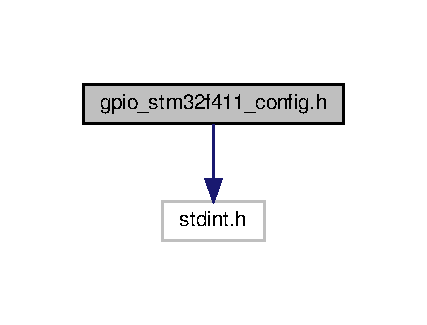
\includegraphics[width=205pt]{gpio__stm32f411__config_8h__incl}
\end{center}
\end{figure}
This graph shows which files directly or indirectly include this file\+:\nopagebreak
\begin{figure}[H]
\begin{center}
\leavevmode
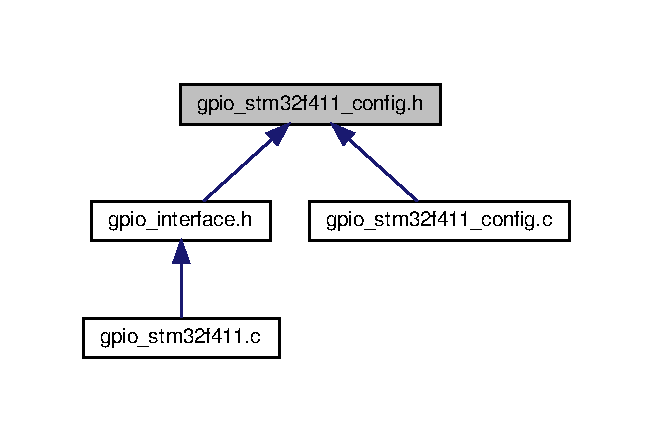
\includegraphics[width=314pt]{gpio__stm32f411__config_8h__dep__incl}
\end{center}
\end{figure}
\subsection*{Data Structures}
\begin{DoxyCompactItemize}
\item 
struct \hyperlink{structgpio__config__t}{gpio\+\_\+config\+\_\+t}
\end{DoxyCompactItemize}
\subsection*{Enumerations}
\begin{DoxyCompactItemize}
\item 
enum \hyperlink{gpio__stm32f411__config_8h_abf6d98e99fb0fb81b56c89f29bd6120e}{gpio\+\_\+pin\+\_\+t} \{ \newline
{\bfseries G\+P\+I\+O\+\_\+\+A\+\_\+0}, 
{\bfseries G\+P\+I\+O\+\_\+\+A\+\_\+1}, 
{\bfseries G\+P\+I\+O\+\_\+\+A\+\_\+2}, 
{\bfseries G\+P\+I\+O\+\_\+\+A\+\_\+3}, 
\newline
{\bfseries G\+P\+I\+O\+\_\+\+A\+\_\+4}, 
{\bfseries G\+P\+I\+O\+\_\+\+A\+\_\+5}, 
{\bfseries G\+P\+I\+O\+\_\+\+A\+\_\+6}, 
{\bfseries G\+P\+I\+O\+\_\+\+A\+\_\+7}, 
\newline
{\bfseries G\+P\+I\+O\+\_\+\+A\+\_\+8}, 
{\bfseries G\+P\+I\+O\+\_\+\+A\+\_\+9}, 
{\bfseries G\+P\+I\+O\+\_\+\+A\+\_\+10}, 
{\bfseries G\+P\+I\+O\+\_\+\+A\+\_\+11}, 
\newline
{\bfseries G\+P\+I\+O\+\_\+\+A\+\_\+12}, 
{\bfseries G\+P\+I\+O\+\_\+\+A\+\_\+13}, 
{\bfseries G\+P\+I\+O\+\_\+\+A\+\_\+14}, 
{\bfseries G\+P\+I\+O\+\_\+\+A\+\_\+15}, 
\newline
{\bfseries G\+P\+I\+O\+\_\+\+B\+\_\+0}, 
{\bfseries G\+P\+I\+O\+\_\+\+B\+\_\+1}, 
{\bfseries G\+P\+I\+O\+\_\+\+B\+\_\+2}, 
{\bfseries G\+P\+I\+O\+\_\+\+B\+\_\+3}, 
\newline
{\bfseries G\+P\+I\+O\+\_\+\+B\+\_\+4}, 
{\bfseries G\+P\+I\+O\+\_\+\+B\+\_\+5}, 
{\bfseries G\+P\+I\+O\+\_\+\+B\+\_\+6}, 
{\bfseries G\+P\+I\+O\+\_\+\+B\+\_\+7}, 
\newline
{\bfseries G\+P\+I\+O\+\_\+\+B\+\_\+8}, 
{\bfseries G\+P\+I\+O\+\_\+\+B\+\_\+9}, 
{\bfseries G\+P\+I\+O\+\_\+\+B\+\_\+10}, 
{\bfseries G\+P\+I\+O\+\_\+\+B\+\_\+11}, 
\newline
{\bfseries G\+P\+I\+O\+\_\+\+B\+\_\+12}, 
{\bfseries G\+P\+I\+O\+\_\+\+B\+\_\+13}, 
{\bfseries G\+P\+I\+O\+\_\+\+B\+\_\+14}, 
{\bfseries G\+P\+I\+O\+\_\+\+B\+\_\+15}, 
\newline
{\bfseries G\+P\+I\+O\+\_\+\+C\+\_\+0}, 
{\bfseries G\+P\+I\+O\+\_\+\+C\+\_\+1}, 
{\bfseries G\+P\+I\+O\+\_\+\+C\+\_\+2}, 
{\bfseries G\+P\+I\+O\+\_\+\+C\+\_\+3}, 
\newline
{\bfseries G\+P\+I\+O\+\_\+\+C\+\_\+4}, 
{\bfseries G\+P\+I\+O\+\_\+\+C\+\_\+5}, 
{\bfseries G\+P\+I\+O\+\_\+\+C\+\_\+6}, 
{\bfseries G\+P\+I\+O\+\_\+\+C\+\_\+7}, 
\newline
{\bfseries G\+P\+I\+O\+\_\+\+C\+\_\+8}, 
{\bfseries G\+P\+I\+O\+\_\+\+C\+\_\+9}, 
{\bfseries G\+P\+I\+O\+\_\+\+C\+\_\+10}, 
{\bfseries G\+P\+I\+O\+\_\+\+C\+\_\+11}, 
\newline
{\bfseries G\+P\+I\+O\+\_\+\+C\+\_\+12}, 
{\bfseries G\+P\+I\+O\+\_\+\+C\+\_\+13}, 
{\bfseries G\+P\+I\+O\+\_\+\+C\+\_\+14}, 
{\bfseries G\+P\+I\+O\+\_\+\+C\+\_\+15}, 
\newline
{\bfseries G\+P\+I\+O\+\_\+\+D\+\_\+0}, 
{\bfseries G\+P\+I\+O\+\_\+\+D\+\_\+1}, 
{\bfseries G\+P\+I\+O\+\_\+\+D\+\_\+2}, 
{\bfseries G\+P\+I\+O\+\_\+\+D\+\_\+3}, 
\newline
{\bfseries G\+P\+I\+O\+\_\+\+D\+\_\+4}, 
{\bfseries G\+P\+I\+O\+\_\+\+D\+\_\+5}, 
{\bfseries G\+P\+I\+O\+\_\+\+D\+\_\+6}, 
{\bfseries G\+P\+I\+O\+\_\+\+D\+\_\+7}, 
\newline
{\bfseries G\+P\+I\+O\+\_\+\+D\+\_\+8}, 
{\bfseries G\+P\+I\+O\+\_\+\+D\+\_\+9}, 
{\bfseries G\+P\+I\+O\+\_\+\+D\+\_\+10}, 
{\bfseries G\+P\+I\+O\+\_\+\+D\+\_\+11}, 
\newline
{\bfseries G\+P\+I\+O\+\_\+\+D\+\_\+12}, 
{\bfseries G\+P\+I\+O\+\_\+\+D\+\_\+13}, 
{\bfseries G\+P\+I\+O\+\_\+\+D\+\_\+14}, 
{\bfseries G\+P\+I\+O\+\_\+\+D\+\_\+15}, 
\newline
{\bfseries G\+P\+I\+O\+\_\+\+E\+\_\+0}, 
{\bfseries G\+P\+I\+O\+\_\+\+E\+\_\+1}, 
{\bfseries G\+P\+I\+O\+\_\+\+E\+\_\+2}, 
{\bfseries G\+P\+I\+O\+\_\+\+E\+\_\+3}, 
\newline
{\bfseries G\+P\+I\+O\+\_\+\+E\+\_\+4}, 
{\bfseries G\+P\+I\+O\+\_\+\+E\+\_\+5}, 
{\bfseries G\+P\+I\+O\+\_\+\+E\+\_\+6}, 
{\bfseries G\+P\+I\+O\+\_\+\+E\+\_\+7}, 
\newline
{\bfseries G\+P\+I\+O\+\_\+\+E\+\_\+8}, 
{\bfseries G\+P\+I\+O\+\_\+\+E\+\_\+9}, 
{\bfseries G\+P\+I\+O\+\_\+\+E\+\_\+10}, 
{\bfseries G\+P\+I\+O\+\_\+\+E\+\_\+11}, 
\newline
{\bfseries G\+P\+I\+O\+\_\+\+E\+\_\+12}, 
{\bfseries G\+P\+I\+O\+\_\+\+E\+\_\+13}, 
{\bfseries G\+P\+I\+O\+\_\+\+E\+\_\+14}, 
{\bfseries G\+P\+I\+O\+\_\+\+E\+\_\+15}, 
\newline
{\bfseries N\+U\+M\+\_\+\+G\+P\+I\+O\+\_\+\+P\+I\+NS}
 \}
\item 
enum \hyperlink{gpio__stm32f411__config_8h_a5e8c50a3dc51d01d0e6bdf2428ee59a7}{gpio\+\_\+pin\+\_\+state\+\_\+t} \{ {\bfseries G\+P\+I\+O\+\_\+\+P\+I\+N\+\_\+\+L\+OW} = 0\+UL, 
{\bfseries G\+P\+I\+O\+\_\+\+P\+I\+N\+\_\+\+H\+I\+GH} = 1\+UL
 \}
\item 
enum \hyperlink{gpio__stm32f411__config_8h_a491a2cbfb4e94f2afcc0d5bdef2dc454}{gpio\+\_\+mode\+\_\+t} \{ \newline
\hyperlink{gpio__stm32f411__config_8h_a491a2cbfb4e94f2afcc0d5bdef2dc454aa1ea38ffc304a6c32480a65b5fec7302}{G\+P\+I\+O\+\_\+\+I\+N\+P\+UT}, 
\hyperlink{gpio__stm32f411__config_8h_a491a2cbfb4e94f2afcc0d5bdef2dc454aa248e73c1faee9c6f072fd91569cf516}{G\+P\+I\+O\+\_\+\+O\+U\+T\+P\+UT}, 
\hyperlink{gpio__stm32f411__config_8h_a491a2cbfb4e94f2afcc0d5bdef2dc454a17fc775975ea5fd3a7d9e61a9ed158d9}{G\+P\+I\+O\+\_\+\+A\+L\+T\+E\+R\+N\+A\+T\+E\+\_\+\+F\+U\+N\+C\+T\+I\+ON}, 
\hyperlink{gpio__stm32f411__config_8h_a491a2cbfb4e94f2afcc0d5bdef2dc454ae8bd62cf000e751ffdce5a9de1c0dcc0}{G\+P\+I\+O\+\_\+\+A\+N\+A\+L\+OG}, 
\newline
\hyperlink{gpio__stm32f411__config_8h_a491a2cbfb4e94f2afcc0d5bdef2dc454ae0ee8a8e757106cefaa2a710b4190062}{G\+P\+I\+O\+\_\+\+M\+A\+X\+\_\+\+M\+O\+D\+E\+\_\+\+O\+P\+T\+I\+O\+NS}
 \}
\item 
enum \hyperlink{gpio__stm32f411__config_8h_ae69599cbb4f87bfc9da21f3db8b0fe3a}{gpio\+\_\+resistor\+\_\+t} \{ \hyperlink{gpio__stm32f411__config_8h_ae69599cbb4f87bfc9da21f3db8b0fe3aa97f95634a424bda4c7b4437a0e4b5f38}{G\+P\+I\+O\+\_\+\+N\+O\+\_\+\+R\+E\+S\+I\+S\+T\+OR}, 
\hyperlink{gpio__stm32f411__config_8h_ae69599cbb4f87bfc9da21f3db8b0fe3aae7d1b2a9078939dd744dd9a7cd61d9df}{G\+P\+I\+O\+\_\+\+P\+U\+L\+L\+\_\+\+UP}, 
\hyperlink{gpio__stm32f411__config_8h_ae69599cbb4f87bfc9da21f3db8b0fe3aa93970a9b4ab92816371682f4e537a8e2}{G\+P\+I\+O\+\_\+\+P\+U\+L\+L\+\_\+\+D\+O\+WN}, 
\hyperlink{gpio__stm32f411__config_8h_ae69599cbb4f87bfc9da21f3db8b0fe3aa39338530834967fdec49448fcda325ab}{G\+P\+I\+O\+\_\+\+M\+A\+X\+\_\+\+R\+E\+S\+I\+S\+T\+O\+R\+\_\+\+O\+P\+T\+I\+O\+NS}
 \}
\item 
enum \hyperlink{gpio__stm32f411__config_8h_a09cae9c54cabb67e47ab4c1200b341c6}{gpio\+\_\+output\+\_\+type\+\_\+t} \{ \hyperlink{gpio__stm32f411__config_8h_a09cae9c54cabb67e47ab4c1200b341c6a2ede6e0f1b50e67e840a93701323c775}{G\+P\+I\+O\+\_\+\+P\+U\+S\+H\+\_\+\+P\+U\+LL}, 
\hyperlink{gpio__stm32f411__config_8h_a09cae9c54cabb67e47ab4c1200b341c6a5b0c623028002305892a4558ef0a6222}{G\+P\+I\+O\+\_\+\+O\+P\+E\+N\+\_\+\+D\+R\+A\+IN}, 
\hyperlink{gpio__stm32f411__config_8h_a09cae9c54cabb67e47ab4c1200b341c6a453c324ad0f7c4c0fcb526e09c430379}{G\+P\+I\+O\+\_\+\+M\+A\+X\+\_\+\+O\+U\+T\+P\+U\+T\+\_\+\+O\+P\+T\+I\+O\+NS}
 \}
\item 
enum \hyperlink{gpio__stm32f411__config_8h_aa8c7c905e73523d86cfed9bd45aa9495}{gpio\+\_\+output\+\_\+speed\+\_\+t} \{ \newline
\hyperlink{gpio__stm32f411__config_8h_aa8c7c905e73523d86cfed9bd45aa9495adad1d99afc424c9903c2116308da5778}{G\+P\+I\+O\+\_\+\+L\+O\+W\+\_\+\+S\+P\+E\+ED}, 
\hyperlink{gpio__stm32f411__config_8h_aa8c7c905e73523d86cfed9bd45aa9495a357cb42172062338fb8a9f316b345082}{G\+P\+I\+O\+\_\+\+M\+E\+D\+\_\+\+S\+P\+E\+ED}, 
\hyperlink{gpio__stm32f411__config_8h_aa8c7c905e73523d86cfed9bd45aa9495a7f887b162032802729cd2f41323a33ff}{G\+P\+I\+O\+\_\+\+F\+A\+S\+T\+\_\+\+S\+P\+E\+ED}, 
\hyperlink{gpio__stm32f411__config_8h_aa8c7c905e73523d86cfed9bd45aa9495adb3d95caeba959c63a9709ca19a9cd04}{G\+P\+I\+O\+\_\+\+H\+I\+G\+H\+\_\+\+S\+P\+E\+ED}, 
\newline
\hyperlink{gpio__stm32f411__config_8h_aa8c7c905e73523d86cfed9bd45aa9495aeafb846c9eb9b0fa2a44628791f32af1}{G\+P\+I\+O\+\_\+\+M\+A\+X\+\_\+\+S\+P\+E\+E\+D\+\_\+\+O\+P\+T\+I\+O\+NS}
 \}
\item 
enum \hyperlink{gpio__stm32f411__config_8h_ac86e130e5617ffe35f2aa1169d8a67c0}{gpio\+\_\+mux\+\_\+t} \{ \newline
{\bfseries G\+P\+I\+O\+\_\+\+A\+F\+\_\+0}, 
{\bfseries G\+P\+I\+O\+\_\+\+A\+F\+\_\+1}, 
{\bfseries G\+P\+I\+O\+\_\+\+A\+F\+\_\+2}, 
{\bfseries G\+P\+I\+O\+\_\+\+A\+F\+\_\+3}, 
\newline
{\bfseries G\+P\+I\+O\+\_\+\+A\+F\+\_\+4}, 
{\bfseries G\+P\+I\+O\+\_\+\+A\+F\+\_\+5}, 
{\bfseries G\+P\+I\+O\+\_\+\+A\+F\+\_\+6}, 
{\bfseries G\+P\+I\+O\+\_\+\+A\+F\+\_\+7}, 
\newline
{\bfseries G\+P\+I\+O\+\_\+\+A\+F\+\_\+8}, 
{\bfseries G\+P\+I\+O\+\_\+\+A\+F\+\_\+9}, 
{\bfseries G\+P\+I\+O\+\_\+\+A\+F\+\_\+10}, 
{\bfseries G\+P\+I\+O\+\_\+\+A\+F\+\_\+11}, 
\newline
{\bfseries G\+P\+I\+O\+\_\+\+A\+F\+\_\+12}, 
{\bfseries G\+P\+I\+O\+\_\+\+A\+F\+\_\+13}, 
{\bfseries G\+P\+I\+O\+\_\+\+A\+F\+\_\+14}, 
{\bfseries G\+P\+I\+O\+\_\+\+A\+F\+\_\+15}, 
\newline
{\bfseries G\+P\+I\+O\+\_\+\+M\+A\+X\+\_\+\+A\+F\+\_\+\+O\+P\+T\+I\+O\+NS}
 \}
\end{DoxyCompactItemize}
\subsection*{Functions}
\begin{DoxyCompactItemize}
\item 
const \hyperlink{structgpio__config__t}{gpio\+\_\+config\+\_\+t} $\ast$ \hyperlink{gpio__stm32f411__config_8h_a2f1150ba6fa738e90abcd72b16507062}{gpio\+\_\+config\+\_\+get} (void)
\end{DoxyCompactItemize}


\subsection{Detailed Description}
machine specific configuration enumerations and structures 



\subsection{Enumeration Type Documentation}
\mbox{\Hypertarget{gpio__stm32f411__config_8h_a491a2cbfb4e94f2afcc0d5bdef2dc454}\label{gpio__stm32f411__config_8h_a491a2cbfb4e94f2afcc0d5bdef2dc454}} 
\index{gpio\+\_\+stm32f411\+\_\+config.\+h@{gpio\+\_\+stm32f411\+\_\+config.\+h}!gpio\+\_\+mode\+\_\+t@{gpio\+\_\+mode\+\_\+t}}
\index{gpio\+\_\+mode\+\_\+t@{gpio\+\_\+mode\+\_\+t}!gpio\+\_\+stm32f411\+\_\+config.\+h@{gpio\+\_\+stm32f411\+\_\+config.\+h}}
\subsubsection{\texorpdfstring{gpio\+\_\+mode\+\_\+t}{gpio\_mode\_t}}
{\footnotesize\ttfamily enum \hyperlink{gpio__stm32f411__config_8h_a491a2cbfb4e94f2afcc0d5bdef2dc454}{gpio\+\_\+mode\+\_\+t}}

Contains all the modes a specific pin can be in. \begin{DoxyEnumFields}{Enumerator}
\raisebox{\heightof{T}}[0pt][0pt]{\index{G\+P\+I\+O\+\_\+\+I\+N\+P\+UT@{G\+P\+I\+O\+\_\+\+I\+N\+P\+UT}!gpio\+\_\+stm32f411\+\_\+config.\+h@{gpio\+\_\+stm32f411\+\_\+config.\+h}}\index{gpio\+\_\+stm32f411\+\_\+config.\+h@{gpio\+\_\+stm32f411\+\_\+config.\+h}!G\+P\+I\+O\+\_\+\+I\+N\+P\+UT@{G\+P\+I\+O\+\_\+\+I\+N\+P\+UT}}}\mbox{\Hypertarget{gpio__stm32f411__config_8h_a491a2cbfb4e94f2afcc0d5bdef2dc454aa1ea38ffc304a6c32480a65b5fec7302}\label{gpio__stm32f411__config_8h_a491a2cbfb4e94f2afcc0d5bdef2dc454aa1ea38ffc304a6c32480a65b5fec7302}} 
G\+P\+I\+O\+\_\+\+I\+N\+P\+UT&The pin functions as a digital input \\
\hline

\raisebox{\heightof{T}}[0pt][0pt]{\index{G\+P\+I\+O\+\_\+\+O\+U\+T\+P\+UT@{G\+P\+I\+O\+\_\+\+O\+U\+T\+P\+UT}!gpio\+\_\+stm32f411\+\_\+config.\+h@{gpio\+\_\+stm32f411\+\_\+config.\+h}}\index{gpio\+\_\+stm32f411\+\_\+config.\+h@{gpio\+\_\+stm32f411\+\_\+config.\+h}!G\+P\+I\+O\+\_\+\+O\+U\+T\+P\+UT@{G\+P\+I\+O\+\_\+\+O\+U\+T\+P\+UT}}}\mbox{\Hypertarget{gpio__stm32f411__config_8h_a491a2cbfb4e94f2afcc0d5bdef2dc454aa248e73c1faee9c6f072fd91569cf516}\label{gpio__stm32f411__config_8h_a491a2cbfb4e94f2afcc0d5bdef2dc454aa248e73c1faee9c6f072fd91569cf516}} 
G\+P\+I\+O\+\_\+\+O\+U\+T\+P\+UT&The pin functions as a digital output \\
\hline

\raisebox{\heightof{T}}[0pt][0pt]{\index{G\+P\+I\+O\+\_\+\+A\+L\+T\+E\+R\+N\+A\+T\+E\+\_\+\+F\+U\+N\+C\+T\+I\+ON@{G\+P\+I\+O\+\_\+\+A\+L\+T\+E\+R\+N\+A\+T\+E\+\_\+\+F\+U\+N\+C\+T\+I\+ON}!gpio\+\_\+stm32f411\+\_\+config.\+h@{gpio\+\_\+stm32f411\+\_\+config.\+h}}\index{gpio\+\_\+stm32f411\+\_\+config.\+h@{gpio\+\_\+stm32f411\+\_\+config.\+h}!G\+P\+I\+O\+\_\+\+A\+L\+T\+E\+R\+N\+A\+T\+E\+\_\+\+F\+U\+N\+C\+T\+I\+ON@{G\+P\+I\+O\+\_\+\+A\+L\+T\+E\+R\+N\+A\+T\+E\+\_\+\+F\+U\+N\+C\+T\+I\+ON}}}\mbox{\Hypertarget{gpio__stm32f411__config_8h_a491a2cbfb4e94f2afcc0d5bdef2dc454a17fc775975ea5fd3a7d9e61a9ed158d9}\label{gpio__stm32f411__config_8h_a491a2cbfb4e94f2afcc0d5bdef2dc454a17fc775975ea5fd3a7d9e61a9ed158d9}} 
G\+P\+I\+O\+\_\+\+A\+L\+T\+E\+R\+N\+A\+T\+E\+\_\+\+F\+U\+N\+C\+T\+I\+ON&The pin is multiplexed to allow another peripheral to control it \begin{DoxySeeAlso}{See also}
\hyperlink{gpio__stm32f411__config_8h_ac86e130e5617ffe35f2aa1169d8a67c0}{gpio\+\_\+mux\+\_\+t} 
\end{DoxySeeAlso}
\\
\hline

\raisebox{\heightof{T}}[0pt][0pt]{\index{G\+P\+I\+O\+\_\+\+A\+N\+A\+L\+OG@{G\+P\+I\+O\+\_\+\+A\+N\+A\+L\+OG}!gpio\+\_\+stm32f411\+\_\+config.\+h@{gpio\+\_\+stm32f411\+\_\+config.\+h}}\index{gpio\+\_\+stm32f411\+\_\+config.\+h@{gpio\+\_\+stm32f411\+\_\+config.\+h}!G\+P\+I\+O\+\_\+\+A\+N\+A\+L\+OG@{G\+P\+I\+O\+\_\+\+A\+N\+A\+L\+OG}}}\mbox{\Hypertarget{gpio__stm32f411__config_8h_a491a2cbfb4e94f2afcc0d5bdef2dc454ae8bd62cf000e751ffdce5a9de1c0dcc0}\label{gpio__stm32f411__config_8h_a491a2cbfb4e94f2afcc0d5bdef2dc454ae8bd62cf000e751ffdce5a9de1c0dcc0}} 
G\+P\+I\+O\+\_\+\+A\+N\+A\+L\+OG&The pin works as an analog, defined by the A\+DC peripheral \\
\hline

\raisebox{\heightof{T}}[0pt][0pt]{\index{G\+P\+I\+O\+\_\+\+M\+A\+X\+\_\+\+M\+O\+D\+E\+\_\+\+O\+P\+T\+I\+O\+NS@{G\+P\+I\+O\+\_\+\+M\+A\+X\+\_\+\+M\+O\+D\+E\+\_\+\+O\+P\+T\+I\+O\+NS}!gpio\+\_\+stm32f411\+\_\+config.\+h@{gpio\+\_\+stm32f411\+\_\+config.\+h}}\index{gpio\+\_\+stm32f411\+\_\+config.\+h@{gpio\+\_\+stm32f411\+\_\+config.\+h}!G\+P\+I\+O\+\_\+\+M\+A\+X\+\_\+\+M\+O\+D\+E\+\_\+\+O\+P\+T\+I\+O\+NS@{G\+P\+I\+O\+\_\+\+M\+A\+X\+\_\+\+M\+O\+D\+E\+\_\+\+O\+P\+T\+I\+O\+NS}}}\mbox{\Hypertarget{gpio__stm32f411__config_8h_a491a2cbfb4e94f2afcc0d5bdef2dc454ae0ee8a8e757106cefaa2a710b4190062}\label{gpio__stm32f411__config_8h_a491a2cbfb4e94f2afcc0d5bdef2dc454ae0ee8a8e757106cefaa2a710b4190062}} 
G\+P\+I\+O\+\_\+\+M\+A\+X\+\_\+\+M\+O\+D\+E\+\_\+\+O\+P\+T\+I\+O\+NS&Redundant extra option. Can be used for assertions in super robust implementations where the strength of enums is in question. \\
\hline

\end{DoxyEnumFields}
\mbox{\Hypertarget{gpio__stm32f411__config_8h_ac86e130e5617ffe35f2aa1169d8a67c0}\label{gpio__stm32f411__config_8h_ac86e130e5617ffe35f2aa1169d8a67c0}} 
\index{gpio\+\_\+stm32f411\+\_\+config.\+h@{gpio\+\_\+stm32f411\+\_\+config.\+h}!gpio\+\_\+mux\+\_\+t@{gpio\+\_\+mux\+\_\+t}}
\index{gpio\+\_\+mux\+\_\+t@{gpio\+\_\+mux\+\_\+t}!gpio\+\_\+stm32f411\+\_\+config.\+h@{gpio\+\_\+stm32f411\+\_\+config.\+h}}
\subsubsection{\texorpdfstring{gpio\+\_\+mux\+\_\+t}{gpio\_mux\_t}}
{\footnotesize\ttfamily enum \hyperlink{gpio__stm32f411__config_8h_ac86e130e5617ffe35f2aa1169d8a67c0}{gpio\+\_\+mux\+\_\+t}}

All alternate function values fed into the 4bit multiplexer. See Figure 17 in R\+M0383 \mbox{\Hypertarget{gpio__stm32f411__config_8h_aa8c7c905e73523d86cfed9bd45aa9495}\label{gpio__stm32f411__config_8h_aa8c7c905e73523d86cfed9bd45aa9495}} 
\index{gpio\+\_\+stm32f411\+\_\+config.\+h@{gpio\+\_\+stm32f411\+\_\+config.\+h}!gpio\+\_\+output\+\_\+speed\+\_\+t@{gpio\+\_\+output\+\_\+speed\+\_\+t}}
\index{gpio\+\_\+output\+\_\+speed\+\_\+t@{gpio\+\_\+output\+\_\+speed\+\_\+t}!gpio\+\_\+stm32f411\+\_\+config.\+h@{gpio\+\_\+stm32f411\+\_\+config.\+h}}
\subsubsection{\texorpdfstring{gpio\+\_\+output\+\_\+speed\+\_\+t}{gpio\_output\_speed\_t}}
{\footnotesize\ttfamily enum \hyperlink{gpio__stm32f411__config_8h_aa8c7c905e73523d86cfed9bd45aa9495}{gpio\+\_\+output\+\_\+speed\+\_\+t}}

Contains speed options for a pin\textquotesingle{}s output. Actual speed is a factor Vdd and capacitor selection. See pages 101-\/102 in the S\+T\+M32\+F411xE datasheet for concrete numbers. All ranges given below are implementation sensitive \begin{DoxyEnumFields}{Enumerator}
\raisebox{\heightof{T}}[0pt][0pt]{\index{G\+P\+I\+O\+\_\+\+L\+O\+W\+\_\+\+S\+P\+E\+ED@{G\+P\+I\+O\+\_\+\+L\+O\+W\+\_\+\+S\+P\+E\+ED}!gpio\+\_\+stm32f411\+\_\+config.\+h@{gpio\+\_\+stm32f411\+\_\+config.\+h}}\index{gpio\+\_\+stm32f411\+\_\+config.\+h@{gpio\+\_\+stm32f411\+\_\+config.\+h}!G\+P\+I\+O\+\_\+\+L\+O\+W\+\_\+\+S\+P\+E\+ED@{G\+P\+I\+O\+\_\+\+L\+O\+W\+\_\+\+S\+P\+E\+ED}}}\mbox{\Hypertarget{gpio__stm32f411__config_8h_aa8c7c905e73523d86cfed9bd45aa9495adad1d99afc424c9903c2116308da5778}\label{gpio__stm32f411__config_8h_aa8c7c905e73523d86cfed9bd45aa9495adad1d99afc424c9903c2116308da5778}} 
G\+P\+I\+O\+\_\+\+L\+O\+W\+\_\+\+S\+P\+E\+ED&Output speed is between 2-\/8\+M\+Hz \\
\hline

\raisebox{\heightof{T}}[0pt][0pt]{\index{G\+P\+I\+O\+\_\+\+M\+E\+D\+\_\+\+S\+P\+E\+ED@{G\+P\+I\+O\+\_\+\+M\+E\+D\+\_\+\+S\+P\+E\+ED}!gpio\+\_\+stm32f411\+\_\+config.\+h@{gpio\+\_\+stm32f411\+\_\+config.\+h}}\index{gpio\+\_\+stm32f411\+\_\+config.\+h@{gpio\+\_\+stm32f411\+\_\+config.\+h}!G\+P\+I\+O\+\_\+\+M\+E\+D\+\_\+\+S\+P\+E\+ED@{G\+P\+I\+O\+\_\+\+M\+E\+D\+\_\+\+S\+P\+E\+ED}}}\mbox{\Hypertarget{gpio__stm32f411__config_8h_aa8c7c905e73523d86cfed9bd45aa9495a357cb42172062338fb8a9f316b345082}\label{gpio__stm32f411__config_8h_aa8c7c905e73523d86cfed9bd45aa9495a357cb42172062338fb8a9f316b345082}} 
G\+P\+I\+O\+\_\+\+M\+E\+D\+\_\+\+S\+P\+E\+ED&Output speed is between 12.\+5-\/50\+M\+Hz \\
\hline

\raisebox{\heightof{T}}[0pt][0pt]{\index{G\+P\+I\+O\+\_\+\+F\+A\+S\+T\+\_\+\+S\+P\+E\+ED@{G\+P\+I\+O\+\_\+\+F\+A\+S\+T\+\_\+\+S\+P\+E\+ED}!gpio\+\_\+stm32f411\+\_\+config.\+h@{gpio\+\_\+stm32f411\+\_\+config.\+h}}\index{gpio\+\_\+stm32f411\+\_\+config.\+h@{gpio\+\_\+stm32f411\+\_\+config.\+h}!G\+P\+I\+O\+\_\+\+F\+A\+S\+T\+\_\+\+S\+P\+E\+ED@{G\+P\+I\+O\+\_\+\+F\+A\+S\+T\+\_\+\+S\+P\+E\+ED}}}\mbox{\Hypertarget{gpio__stm32f411__config_8h_aa8c7c905e73523d86cfed9bd45aa9495a7f887b162032802729cd2f41323a33ff}\label{gpio__stm32f411__config_8h_aa8c7c905e73523d86cfed9bd45aa9495a7f887b162032802729cd2f41323a33ff}} 
G\+P\+I\+O\+\_\+\+F\+A\+S\+T\+\_\+\+S\+P\+E\+ED&Output speed is between 25-\/100\+M\+Hz \\
\hline

\raisebox{\heightof{T}}[0pt][0pt]{\index{G\+P\+I\+O\+\_\+\+H\+I\+G\+H\+\_\+\+S\+P\+E\+ED@{G\+P\+I\+O\+\_\+\+H\+I\+G\+H\+\_\+\+S\+P\+E\+ED}!gpio\+\_\+stm32f411\+\_\+config.\+h@{gpio\+\_\+stm32f411\+\_\+config.\+h}}\index{gpio\+\_\+stm32f411\+\_\+config.\+h@{gpio\+\_\+stm32f411\+\_\+config.\+h}!G\+P\+I\+O\+\_\+\+H\+I\+G\+H\+\_\+\+S\+P\+E\+ED@{G\+P\+I\+O\+\_\+\+H\+I\+G\+H\+\_\+\+S\+P\+E\+ED}}}\mbox{\Hypertarget{gpio__stm32f411__config_8h_aa8c7c905e73523d86cfed9bd45aa9495adb3d95caeba959c63a9709ca19a9cd04}\label{gpio__stm32f411__config_8h_aa8c7c905e73523d86cfed9bd45aa9495adb3d95caeba959c63a9709ca19a9cd04}} 
G\+P\+I\+O\+\_\+\+H\+I\+G\+H\+\_\+\+S\+P\+E\+ED&Output speed is between 50-\/100\+M\+Hz \\
\hline

\raisebox{\heightof{T}}[0pt][0pt]{\index{G\+P\+I\+O\+\_\+\+M\+A\+X\+\_\+\+S\+P\+E\+E\+D\+\_\+\+O\+P\+T\+I\+O\+NS@{G\+P\+I\+O\+\_\+\+M\+A\+X\+\_\+\+S\+P\+E\+E\+D\+\_\+\+O\+P\+T\+I\+O\+NS}!gpio\+\_\+stm32f411\+\_\+config.\+h@{gpio\+\_\+stm32f411\+\_\+config.\+h}}\index{gpio\+\_\+stm32f411\+\_\+config.\+h@{gpio\+\_\+stm32f411\+\_\+config.\+h}!G\+P\+I\+O\+\_\+\+M\+A\+X\+\_\+\+S\+P\+E\+E\+D\+\_\+\+O\+P\+T\+I\+O\+NS@{G\+P\+I\+O\+\_\+\+M\+A\+X\+\_\+\+S\+P\+E\+E\+D\+\_\+\+O\+P\+T\+I\+O\+NS}}}\mbox{\Hypertarget{gpio__stm32f411__config_8h_aa8c7c905e73523d86cfed9bd45aa9495aeafb846c9eb9b0fa2a44628791f32af1}\label{gpio__stm32f411__config_8h_aa8c7c905e73523d86cfed9bd45aa9495aeafb846c9eb9b0fa2a44628791f32af1}} 
G\+P\+I\+O\+\_\+\+M\+A\+X\+\_\+\+S\+P\+E\+E\+D\+\_\+\+O\+P\+T\+I\+O\+NS&Redundant extra option. Can be used for assertions in super robust implementations where the strength of enums is in question. \\
\hline

\end{DoxyEnumFields}
\mbox{\Hypertarget{gpio__stm32f411__config_8h_a09cae9c54cabb67e47ab4c1200b341c6}\label{gpio__stm32f411__config_8h_a09cae9c54cabb67e47ab4c1200b341c6}} 
\index{gpio\+\_\+stm32f411\+\_\+config.\+h@{gpio\+\_\+stm32f411\+\_\+config.\+h}!gpio\+\_\+output\+\_\+type\+\_\+t@{gpio\+\_\+output\+\_\+type\+\_\+t}}
\index{gpio\+\_\+output\+\_\+type\+\_\+t@{gpio\+\_\+output\+\_\+type\+\_\+t}!gpio\+\_\+stm32f411\+\_\+config.\+h@{gpio\+\_\+stm32f411\+\_\+config.\+h}}
\subsubsection{\texorpdfstring{gpio\+\_\+output\+\_\+type\+\_\+t}{gpio\_output\_type\_t}}
{\footnotesize\ttfamily enum \hyperlink{gpio__stm32f411__config_8h_a09cae9c54cabb67e47ab4c1200b341c6}{gpio\+\_\+output\+\_\+type\+\_\+t}}

Defines the electrical behaviour of an output pin. \begin{DoxyEnumFields}{Enumerator}
\raisebox{\heightof{T}}[0pt][0pt]{\index{G\+P\+I\+O\+\_\+\+P\+U\+S\+H\+\_\+\+P\+U\+LL@{G\+P\+I\+O\+\_\+\+P\+U\+S\+H\+\_\+\+P\+U\+LL}!gpio\+\_\+stm32f411\+\_\+config.\+h@{gpio\+\_\+stm32f411\+\_\+config.\+h}}\index{gpio\+\_\+stm32f411\+\_\+config.\+h@{gpio\+\_\+stm32f411\+\_\+config.\+h}!G\+P\+I\+O\+\_\+\+P\+U\+S\+H\+\_\+\+P\+U\+LL@{G\+P\+I\+O\+\_\+\+P\+U\+S\+H\+\_\+\+P\+U\+LL}}}\mbox{\Hypertarget{gpio__stm32f411__config_8h_a09cae9c54cabb67e47ab4c1200b341c6a2ede6e0f1b50e67e840a93701323c775}\label{gpio__stm32f411__config_8h_a09cae9c54cabb67e47ab4c1200b341c6a2ede6e0f1b50e67e840a93701323c775}} 
G\+P\+I\+O\+\_\+\+P\+U\+S\+H\+\_\+\+P\+U\+LL&The pin can drive to electrical defined 1 and 0 (Vdd and G\+ND) \\
\hline

\raisebox{\heightof{T}}[0pt][0pt]{\index{G\+P\+I\+O\+\_\+\+O\+P\+E\+N\+\_\+\+D\+R\+A\+IN@{G\+P\+I\+O\+\_\+\+O\+P\+E\+N\+\_\+\+D\+R\+A\+IN}!gpio\+\_\+stm32f411\+\_\+config.\+h@{gpio\+\_\+stm32f411\+\_\+config.\+h}}\index{gpio\+\_\+stm32f411\+\_\+config.\+h@{gpio\+\_\+stm32f411\+\_\+config.\+h}!G\+P\+I\+O\+\_\+\+O\+P\+E\+N\+\_\+\+D\+R\+A\+IN@{G\+P\+I\+O\+\_\+\+O\+P\+E\+N\+\_\+\+D\+R\+A\+IN}}}\mbox{\Hypertarget{gpio__stm32f411__config_8h_a09cae9c54cabb67e47ab4c1200b341c6a5b0c623028002305892a4558ef0a6222}\label{gpio__stm32f411__config_8h_a09cae9c54cabb67e47ab4c1200b341c6a5b0c623028002305892a4558ef0a6222}} 
G\+P\+I\+O\+\_\+\+O\+P\+E\+N\+\_\+\+D\+R\+A\+IN&The pin can only drive to G\+ND. Output options are undefined and 0. \\
\hline

\raisebox{\heightof{T}}[0pt][0pt]{\index{G\+P\+I\+O\+\_\+\+M\+A\+X\+\_\+\+O\+U\+T\+P\+U\+T\+\_\+\+O\+P\+T\+I\+O\+NS@{G\+P\+I\+O\+\_\+\+M\+A\+X\+\_\+\+O\+U\+T\+P\+U\+T\+\_\+\+O\+P\+T\+I\+O\+NS}!gpio\+\_\+stm32f411\+\_\+config.\+h@{gpio\+\_\+stm32f411\+\_\+config.\+h}}\index{gpio\+\_\+stm32f411\+\_\+config.\+h@{gpio\+\_\+stm32f411\+\_\+config.\+h}!G\+P\+I\+O\+\_\+\+M\+A\+X\+\_\+\+O\+U\+T\+P\+U\+T\+\_\+\+O\+P\+T\+I\+O\+NS@{G\+P\+I\+O\+\_\+\+M\+A\+X\+\_\+\+O\+U\+T\+P\+U\+T\+\_\+\+O\+P\+T\+I\+O\+NS}}}\mbox{\Hypertarget{gpio__stm32f411__config_8h_a09cae9c54cabb67e47ab4c1200b341c6a453c324ad0f7c4c0fcb526e09c430379}\label{gpio__stm32f411__config_8h_a09cae9c54cabb67e47ab4c1200b341c6a453c324ad0f7c4c0fcb526e09c430379}} 
G\+P\+I\+O\+\_\+\+M\+A\+X\+\_\+\+O\+U\+T\+P\+U\+T\+\_\+\+O\+P\+T\+I\+O\+NS&Redundant extra option. Can be used for assertions in super robust implementations where the strength of enums is in question. \\
\hline

\end{DoxyEnumFields}
\mbox{\Hypertarget{gpio__stm32f411__config_8h_a5e8c50a3dc51d01d0e6bdf2428ee59a7}\label{gpio__stm32f411__config_8h_a5e8c50a3dc51d01d0e6bdf2428ee59a7}} 
\index{gpio\+\_\+stm32f411\+\_\+config.\+h@{gpio\+\_\+stm32f411\+\_\+config.\+h}!gpio\+\_\+pin\+\_\+state\+\_\+t@{gpio\+\_\+pin\+\_\+state\+\_\+t}}
\index{gpio\+\_\+pin\+\_\+state\+\_\+t@{gpio\+\_\+pin\+\_\+state\+\_\+t}!gpio\+\_\+stm32f411\+\_\+config.\+h@{gpio\+\_\+stm32f411\+\_\+config.\+h}}
\subsubsection{\texorpdfstring{gpio\+\_\+pin\+\_\+state\+\_\+t}{gpio\_pin\_state\_t}}
{\footnotesize\ttfamily enum \hyperlink{gpio__stm32f411__config_8h_a5e8c50a3dc51d01d0e6bdf2428ee59a7}{gpio\+\_\+pin\+\_\+state\+\_\+t}}

Contains both active states a pin can be in. Actual electrical behaviour depends on push-\/pull/open drain settings. \mbox{\Hypertarget{gpio__stm32f411__config_8h_abf6d98e99fb0fb81b56c89f29bd6120e}\label{gpio__stm32f411__config_8h_abf6d98e99fb0fb81b56c89f29bd6120e}} 
\index{gpio\+\_\+stm32f411\+\_\+config.\+h@{gpio\+\_\+stm32f411\+\_\+config.\+h}!gpio\+\_\+pin\+\_\+t@{gpio\+\_\+pin\+\_\+t}}
\index{gpio\+\_\+pin\+\_\+t@{gpio\+\_\+pin\+\_\+t}!gpio\+\_\+stm32f411\+\_\+config.\+h@{gpio\+\_\+stm32f411\+\_\+config.\+h}}
\subsubsection{\texorpdfstring{gpio\+\_\+pin\+\_\+t}{gpio\_pin\_t}}
{\footnotesize\ttfamily enum \hyperlink{gpio__stm32f411__config_8h_abf6d98e99fb0fb81b56c89f29bd6120e}{gpio\+\_\+pin\+\_\+t}}

Contains all of the gpio pins on all of the ports. Intermediary calculations are used to separate port and pins. \mbox{\Hypertarget{gpio__stm32f411__config_8h_ae69599cbb4f87bfc9da21f3db8b0fe3a}\label{gpio__stm32f411__config_8h_ae69599cbb4f87bfc9da21f3db8b0fe3a}} 
\index{gpio\+\_\+stm32f411\+\_\+config.\+h@{gpio\+\_\+stm32f411\+\_\+config.\+h}!gpio\+\_\+resistor\+\_\+t@{gpio\+\_\+resistor\+\_\+t}}
\index{gpio\+\_\+resistor\+\_\+t@{gpio\+\_\+resistor\+\_\+t}!gpio\+\_\+stm32f411\+\_\+config.\+h@{gpio\+\_\+stm32f411\+\_\+config.\+h}}
\subsubsection{\texorpdfstring{gpio\+\_\+resistor\+\_\+t}{gpio\_resistor\_t}}
{\footnotesize\ttfamily enum \hyperlink{gpio__stm32f411__config_8h_ae69599cbb4f87bfc9da21f3db8b0fe3a}{gpio\+\_\+resistor\+\_\+t}}

Contains the resistor options over a pin for both input and output modes. \begin{DoxyEnumFields}{Enumerator}
\raisebox{\heightof{T}}[0pt][0pt]{\index{G\+P\+I\+O\+\_\+\+N\+O\+\_\+\+R\+E\+S\+I\+S\+T\+OR@{G\+P\+I\+O\+\_\+\+N\+O\+\_\+\+R\+E\+S\+I\+S\+T\+OR}!gpio\+\_\+stm32f411\+\_\+config.\+h@{gpio\+\_\+stm32f411\+\_\+config.\+h}}\index{gpio\+\_\+stm32f411\+\_\+config.\+h@{gpio\+\_\+stm32f411\+\_\+config.\+h}!G\+P\+I\+O\+\_\+\+N\+O\+\_\+\+R\+E\+S\+I\+S\+T\+OR@{G\+P\+I\+O\+\_\+\+N\+O\+\_\+\+R\+E\+S\+I\+S\+T\+OR}}}\mbox{\Hypertarget{gpio__stm32f411__config_8h_ae69599cbb4f87bfc9da21f3db8b0fe3aa97f95634a424bda4c7b4437a0e4b5f38}\label{gpio__stm32f411__config_8h_ae69599cbb4f87bfc9da21f3db8b0fe3aa97f95634a424bda4c7b4437a0e4b5f38}} 
G\+P\+I\+O\+\_\+\+N\+O\+\_\+\+R\+E\+S\+I\+S\+T\+OR&No resistor. Pin is undefined unless driven actively \\
\hline

\raisebox{\heightof{T}}[0pt][0pt]{\index{G\+P\+I\+O\+\_\+\+P\+U\+L\+L\+\_\+\+UP@{G\+P\+I\+O\+\_\+\+P\+U\+L\+L\+\_\+\+UP}!gpio\+\_\+stm32f411\+\_\+config.\+h@{gpio\+\_\+stm32f411\+\_\+config.\+h}}\index{gpio\+\_\+stm32f411\+\_\+config.\+h@{gpio\+\_\+stm32f411\+\_\+config.\+h}!G\+P\+I\+O\+\_\+\+P\+U\+L\+L\+\_\+\+UP@{G\+P\+I\+O\+\_\+\+P\+U\+L\+L\+\_\+\+UP}}}\mbox{\Hypertarget{gpio__stm32f411__config_8h_ae69599cbb4f87bfc9da21f3db8b0fe3aae7d1b2a9078939dd744dd9a7cd61d9df}\label{gpio__stm32f411__config_8h_ae69599cbb4f87bfc9da21f3db8b0fe3aae7d1b2a9078939dd744dd9a7cd61d9df}} 
G\+P\+I\+O\+\_\+\+P\+U\+L\+L\+\_\+\+UP&Pull up resistor over pin. Will default to high unless driven \\
\hline

\raisebox{\heightof{T}}[0pt][0pt]{\index{G\+P\+I\+O\+\_\+\+P\+U\+L\+L\+\_\+\+D\+O\+WN@{G\+P\+I\+O\+\_\+\+P\+U\+L\+L\+\_\+\+D\+O\+WN}!gpio\+\_\+stm32f411\+\_\+config.\+h@{gpio\+\_\+stm32f411\+\_\+config.\+h}}\index{gpio\+\_\+stm32f411\+\_\+config.\+h@{gpio\+\_\+stm32f411\+\_\+config.\+h}!G\+P\+I\+O\+\_\+\+P\+U\+L\+L\+\_\+\+D\+O\+WN@{G\+P\+I\+O\+\_\+\+P\+U\+L\+L\+\_\+\+D\+O\+WN}}}\mbox{\Hypertarget{gpio__stm32f411__config_8h_ae69599cbb4f87bfc9da21f3db8b0fe3aa93970a9b4ab92816371682f4e537a8e2}\label{gpio__stm32f411__config_8h_ae69599cbb4f87bfc9da21f3db8b0fe3aa93970a9b4ab92816371682f4e537a8e2}} 
G\+P\+I\+O\+\_\+\+P\+U\+L\+L\+\_\+\+D\+O\+WN&Pull down resistor over pin. Will default to low unless driven \\
\hline

\raisebox{\heightof{T}}[0pt][0pt]{\index{G\+P\+I\+O\+\_\+\+M\+A\+X\+\_\+\+R\+E\+S\+I\+S\+T\+O\+R\+\_\+\+O\+P\+T\+I\+O\+NS@{G\+P\+I\+O\+\_\+\+M\+A\+X\+\_\+\+R\+E\+S\+I\+S\+T\+O\+R\+\_\+\+O\+P\+T\+I\+O\+NS}!gpio\+\_\+stm32f411\+\_\+config.\+h@{gpio\+\_\+stm32f411\+\_\+config.\+h}}\index{gpio\+\_\+stm32f411\+\_\+config.\+h@{gpio\+\_\+stm32f411\+\_\+config.\+h}!G\+P\+I\+O\+\_\+\+M\+A\+X\+\_\+\+R\+E\+S\+I\+S\+T\+O\+R\+\_\+\+O\+P\+T\+I\+O\+NS@{G\+P\+I\+O\+\_\+\+M\+A\+X\+\_\+\+R\+E\+S\+I\+S\+T\+O\+R\+\_\+\+O\+P\+T\+I\+O\+NS}}}\mbox{\Hypertarget{gpio__stm32f411__config_8h_ae69599cbb4f87bfc9da21f3db8b0fe3aa39338530834967fdec49448fcda325ab}\label{gpio__stm32f411__config_8h_ae69599cbb4f87bfc9da21f3db8b0fe3aa39338530834967fdec49448fcda325ab}} 
G\+P\+I\+O\+\_\+\+M\+A\+X\+\_\+\+R\+E\+S\+I\+S\+T\+O\+R\+\_\+\+O\+P\+T\+I\+O\+NS&Redundant extra option. Can be used for assertions in super robust where the strength of enums is in question. \\
\hline

\end{DoxyEnumFields}


\subsection{Function Documentation}
\mbox{\Hypertarget{gpio__stm32f411__config_8h_a2f1150ba6fa738e90abcd72b16507062}\label{gpio__stm32f411__config_8h_a2f1150ba6fa738e90abcd72b16507062}} 
\index{gpio\+\_\+stm32f411\+\_\+config.\+h@{gpio\+\_\+stm32f411\+\_\+config.\+h}!gpio\+\_\+config\+\_\+get@{gpio\+\_\+config\+\_\+get}}
\index{gpio\+\_\+config\+\_\+get@{gpio\+\_\+config\+\_\+get}!gpio\+\_\+stm32f411\+\_\+config.\+h@{gpio\+\_\+stm32f411\+\_\+config.\+h}}
\subsubsection{\texorpdfstring{gpio\+\_\+config\+\_\+get()}{gpio\_config\_get()}}
{\footnotesize\ttfamily const \hyperlink{structgpio__config__t}{gpio\+\_\+config\+\_\+t}$\ast$ gpio\+\_\+config\+\_\+get (\begin{DoxyParamCaption}\item[{void}]{ }\end{DoxyParamCaption})}

{\bfseries Description\+:} Retrieves the config table for the gpio peripheral, normally hidden statically within the config.\+c file.

P\+R\+E-\/\+C\+O\+N\+D\+I\+T\+I\+ON\+: The config table has been populated/exists with a size greater than 0.

P\+O\+S\+T-\/\+C\+O\+N\+D\+I\+T\+I\+ON\+: The returned value points to the base of the config table

\begin{DoxyReturn}{Returns}
const \hyperlink{structgpio__config__t}{gpio\+\_\+config\+\_\+t} $\ast$
\end{DoxyReturn}
{\bfseries Example\+:} 


\begin{DoxyCode}
\textcolor{keyword}{const} \hyperlink{structgpio__config__t}{gpio\_config\_t} gpio\_config\_table = \hyperlink{gpio__stm32f411__config_8c_a2f1150ba6fa738e90abcd72b16507062}{gpio\_config\_get}(\textcolor{keywordtype}{void});
\hyperlink{gpio__interface_8h_a19bc61b9832a2879bc1c8953dcfae407}{gpio\_init}(gpio\_config\_table);
\end{DoxyCode}


\begin{DoxySeeAlso}{See also}
\hyperlink{gpio__stm32f411_8c_a19bc61b9832a2879bc1c8953dcfae407}{gpio\+\_\+init}
\end{DoxySeeAlso}
~\newline
{\bfseries  -\/ C\+H\+A\+N\+GE H\+I\+S\+T\+O\+RY -\/ }

\tabulinesep=1mm
\begin{longtabu} spread 0pt [c]{*{4}{|X[-1]}|}
\hline
Date &Software Version &Initials &Description  \\\cline{1-4}
\end{longtabu}
~\newline
~\newline
 

 
%--- End generated contents ---

% Index
\backmatter
\newpage
\phantomsection
\clearemptydoublepage
\addcontentsline{toc}{chapter}{Index}
\printindex

\end{document}
